% This is samplepaper.tex, a sample chapter demonstrating the
% LLNCS macro package for Springer Computer Science proceedings;
% Version 2.20 of 2017/10/04
%
\documentclass[runningheads]{llncs}
%
\usepackage{caption}  % For custom captions\usepackage{cite}     % For handling citations
\usepackage{amsmath}  % For mathematical features
\usepackage{graphicx}
\usepackage{booktabs}

\usepackage[colorlinks=true, urlcolor=blue, linkcolor=black]{hyperref}
% Used for displaying a sample figure. If possible, figure files should
% be included in EPS format.
%
% If you use the hyperref package, please uncomment the following line
% to display URLs in blue roman font according to Springer's eBook style:
% \renewcommand\UrlFont{\color{blue}\rmfamily}



\begin{document}
%
\title{Stroke Prediction Capstone Project}
%
%\titlerunning{Abbreviated paper title}
% If the paper title is too long for the running head, you can set
% an abbreviated paper title here
%
\author{Alvaro Quintero Gonzalez}
%
\authorrunning{A. Quintero Gonzalez.}
% First names are abbreviated in the running head.
% If there are more than two authors, 'et al.' is used.
%
\institute{Northwest Missouri State University, Maryville MO 64468, USA \\
\email{S573928@nwmissouri.edu and alvaroquintero28@yahoo.com}\\
}
%
\maketitle              % typeset the header of the contribution
%
\begin{abstract}
Stroke prediction is a critical area of research in healthcare, aiming to enhance preventative strategies and improve patient outcomes. This study investigates a comprehensive dataset collected from various healthcare sources, consisting of demographic, clinical, and lifestyle factors associated with stroke risk. The dataset encompasses attributes such as age, gender, blood pressure, cholesterol levels, body mass index (BMI), and lifestyle habits. Utilizing machine learning algorithms, we apply classification techniques—including logistic regression, decision trees, and random forests—to identify significant predictors of stroke occurrence. Analysis reveals that key factors such as hypertension, diabetes, and smoking significantly increase stroke risk, while regular physical activity acts as a protective measure. The insights gained from this study can guide healthcare professionals in stratifying patients based on their risk profiles and recommending tailored preventative measures. Additionally, findings emphasized the importance of addressing modifiable risk factors in public health initiatives. This research not only contributes to the existing body of literature on stroke prediction but also underscores the potential for machine learning to revolutionize patient care and stroke prevention strategies in clinical practice. 

\keywords{Stroke Prediction \and Preventative Strategies \and Demographic Factors \and Predictive Modeling \and Machine Learning Algorithms}
\end{abstract}
%
%
%
\section{Introduction}

Strokes are a major health concern globally, recognized as one of the leading causes of disability and death. Occurring when blood flow to the brain is disrupted, it can lead to significant physical, cognitive, and emotional impairments in affected individuals. \cite{kaur2022retracted} The impact of strokes extends beyond the individual, affecting families and communities, and placing a substantial strain on healthcare systems. With the rising incidence of strokes associated with aging populations and the increasing prevalence of risk factors such as hypertension, obesity, and diabetes, there is an urgent need to focus on effective stroke prevention strategies. Prevention requires a multifaceted approach that includes public education, early identification of risk factors, and lifestyle modifications. Simple changes, such as adopting a balanced diet, engaging in regular physical activity, and managing underlying health conditions, can greatly reduce an individual's risk of stroke.\cite{doi:10.1161/STR.0000000000000375} Moreover, healthcare providers must play an active role in raising awareness about stroke prevention and ensuring that at-risk patients receive appropriate screenings and interventions. By promoting a comprehensive understanding of stroke risk factors, we can empower individuals to take charge of their health. \cite{sirisha2021awareness} This proactive approach not only aims to reduce the frequency of strokes but also facilitates overall public health awareness, fostering healthier communities. As advances in knowledge and strategies for stroke prevention, we can work towards a future where strokes are less frequent and their consequences are minimized \cite{sirisha2021awareness}.

\subsection{Define the Problem and Goals of This Capstone Project} 
This section discusses the goals of the proposed project. The primary focus of this capstone project is to develop a comprehensive understanding of stroke prediction and prevention strategies using data-driven approaches. Main goal consist of identifying key risk factors. By applying statistical analysis and machine learning techniques, it will determine which variables are most predictive of stroke occurrence. Further focus will evaluate performance of developed models in predicting stroke events, thereby providing valuable insights for early intervention. The project will propose targeted preventive strategies that can be implemented in community health programs therefore enhancing greater public awareness.

\subsubsection*{Project Links}
Key resources for this project provided below:

\begin{itemize}
    \item \href{https://github.com/alvaroquintero28/Capstone-Project-Report}{Capstone-Project-Report GitHub}
    \item \href{https://es.overleaf.com/read/zqgzcfntnwbz#9bc8ce}
    {Capstone Project Report Overleaf}
\end{itemize}

\subsection{The following are the phases of project implementation}

\begin{enumerate}
    \item Define the Problem and Objectives
    \begin{enumerate}
        \item Clearly articulate the specific questions and objectives of the analysis, focusing on how heart disease predictions can improve preventive measures for stroke patients.
         \item Identify key performance indicators to measure the success of the project. 
    \end{enumerate}

\item  Literature Review and Background Research
\begin{enumerate}
    \item Conduct a thorough review of existing literature on heart disease, stroke rehabilitation, and predictive analytics in healthcare. 
    \item Gather insights into current best practices and identify gaps in the existing research that your project can address. 
\end{enumerate}

\item Data Collection
\begin{enumerate}
    \item Search for relevant datasets using the identified sources (e.g., ProjectPro, American Journal of Medicine) focusing on: 
    \begin{enumerate}
        \item Patient demographics 
        \item Medical history related to heart disease and strokes 
        \item Lifestyle factors (e.g., diet, exercise) 
        \item Laboratory test results (e.g., cholesterol levels, blood pressure) 
    \end{enumerate}
    \item Ensure that the data is reliable, accurate, and representative of the population of study. 
\end{enumerate}

\item Data Pre-processing
    \begin{enumerate}
        \item Clean the data by handling missing values, outliers, and inconsistencies. 
        \item Perform data normalization or standardization if necessary. 
        \item Encode categorical variables to facilitate analysis in machine learning models. 
    \end {enumerate}
    
\item  Exploratory Data Analysis (EDA)
    \begin{enumerate}
        \item Analyze the dataset to uncover patterns and relationships between variables. 
        \item Use visualizations (graphs, plots) to represent findings and identify key risk factors associated with heart disease in stroke patients. 
        \item Identify and select the most relevant features that influence heart disease predictions. 
        \item Use techniques like correlation analysis, recursive feature elimination (RFE), or machine learning algorithms to enhance feature selection. 
    \end{enumerate}
    
\item Model Development
    \begin{enumerate}
        \item Choose appropriate machine learning models for prediction 
            \begin{enumerate}
                \item Logistic Regression
                \item Decision Trees 
                \item Random Forest 
                \item Support Vector Machines 
                \item Neural Networks 
            \end{enumerate}
        \item Split the dataset into training and testing sets for model evaluation. 
        \item Train the selected models on training dataset. 
        \item Optimize model performance using techniques like hyperparameter tuning and cross-validation to prevent overfitting. 
        \item Assess the accuracy and effectiveness of the models using the testing dataset. 
        \item Use evaluation metrics such as accuracy, precision, recall, F1 score, and the ROC-AUC curve to measure performance. 
        \item Compare the performance of each model for best selection.
\end{enumerate}

\item Conclusion
\begin{enumerate}
    \item Interpret Results
        \begin{enumerate}
            \item Analyze the results of the best-performing model to understand the impact of various factors on heart disease predictions. 
            \item Provide actionable insights and recommendations for preventing heart disease in stroke patients based on the findings. 
        \end{enumerate}
\item Discussion of the limitations
\item Ideas for future work.
\end{enumerate}

\section{Literature Review and Background Research}
Numerous studies have identified effective preventive measures for reducing the risk of stroke, emphasizing both management of hypertension and lifestyle interventions. \cite{sirisha2021awareness} Hypertension is the most significant modifiable risk factor for stroke, and studies have shown that controlling blood pressure through lifestyle changes, such as a healthy diet, regular physical activity, reducing sodium intake, smoking cessation, and adhering to prescribed antihypertensive medications can significantly lower the likelihood of experiencing a stroke. \cite{doi:10.1161/STR.0000000000000375} Maintaining blood pressure within a normal range (typically less than 120/80 mmHg) is crucial in preventing both ischemic and hemorrhagic strokes, making it the most critical focus in stroke prevention efforts. \cite{doi:10.1161/STR.0000000000000375} Combined, these research findings underscore the importance of a multifaceted approach to stroke prevention that integrates medical treatment with proactive lifestyle changes.

\subsection{Limitations}
The healthcare stroke prevention dataset and the well-being and lifestyle dataset each have inherent limitations that may affect the comprehensiveness and applicability of their findings. Firstly, the stroke prevention dataset may suffer from issues related to sample size and demographic representation, potentially limiting the generalizability of the results across diverse populations. Additionally, the accuracy of self-reported data regarding lifestyle factors in the well-being and lifestyle dataset may be compromised by social desirability bias, where participants might under-report unhealthy behaviors or exaggerate healthy ones. Furthermore, the transient nature of lifestyle habits makes it challenging to capture accurate and stable data over time, potentially leading to discrepancies in understanding long-term behavior trends.

\section{Data}
Data collection for this analysis involved two comprehensive datasets sourced from Kaggle: the Wellbeing and Lifestyle Data and the Healthcare Dataset on Stroke Data. The Wellbeing and Lifestyle Data dataset encompasses a variety of factors influencing individual health and well-being, such as lifestyle choices. It features demographic information, including age, gender, and socioeconomic status, facilitating an understanding of how these variables correlate with reported well-being outcomes. The Healthcare Dataset and Stroke Data, on the other hand, presents critical health metrics and conditions related to stroke incidents among patients. By merging insights from these two datasets, a more comprehensive picture of lifestyle influences on health outcomes can be constructed, enabling a deeper exploration of the relationships between well-being, lifestyle choices, and stroke risk.


\subsection{Dataset Variable Attributes}

The following tables summarize the original data attributes, including their descriptions, data types, and possible values prior to any data cleaning. These attributes are essential for understanding the collected data and are crucial for any subsequent analysis.

\clearpage
\begin{table}[ht]
\centering
\caption{Attributes, Descriptions, and Possible Values from Healthcare Dataset}
\label{tab:healthcare_data_attributes}
\begin{tabular}{|l|p{5cm}|p{4cm}|}
\hline
\textbf{Attribute} & \textbf{Description} & \textbf{Possible Values} \\ 
\hline
\textbf{id} & Unique identifier for each patient & Whole numbers \\ 
\hline
\textbf{gender} & Gender of the patient & "Male", "Female", "Other" \\ 
\hline
\textbf{age} & Age of the patient in years & Whole numbers (e.g., 0, 1, 25, 60) \\ 
\hline
\textbf{hypertension} & Indicates if the patient has hypertension & 0 (No), 1 (Yes) \\ 
\hline
\textbf{heart\_disease} & Indicates if the patient has heart disease & 0 (No), 1 (Yes) \\ 
\hline
\textbf{ever\_married} & Indicates if the patient has ever been married & "Yes", "No" \\ 
\hline
\textbf{work\_type} & Type of employment of the patient & "Children", "Govt job", "Self-employed", "Private", "Never worked" \\ 
\hline
\textbf{Residence\_type} & Type of residence of the patient & "Urban", "Rural" \\ 
\hline
\textbf{avg\_glucose\_level} & Average glucose level of the patient & Positive floats (e.g., 70.0, 220.0) \\ 
\hline
\textbf{bmi} & Body Mass Index of the patient & Positive floats (e.g., 18.5, 30.0) or "N/A" \\ 
\hline
\textbf{smoking\_status} & Indicates the smoking status of the patient & "formerly smoked", "smokes", "never smoked", "Unknown" \\ 
\hline
\textbf{stroke} & Indicates if the patient has had a stroke & 0 (No), 1 (Yes) \\ 
\hline
\end{tabular}
\end{table}

\clearpage

\begin{table}[ht]
\centering
\caption{Attributes, Descriptions, and Possible Values from Work-Life Balance Dataset}
\label{tab:work_life_balance_attributes}
\begin{tabular}{|l|p{5cm}|p{4cm}|}
\hline
\textbf{Attribute} & \textbf{Description} & \textbf{Possible Values} \\ 
\hline
\textbf{Timestamp} & Date of the record entry & Date format (e.g., "7/7/15") \\ 
\hline
\textbf{FRUITS\_VEGGIES} & Number of servings of fruits and vegetables consumed daily & Whole numbers (e.g., 0, 1, 2, 10) \\ 
\hline
\textbf{DAILY\_STRESS} & Daily stress level rating & Whole numbers (e.g., 1 to 10) \\ 
\hline
\textbf{PLACES\_VISITED} & Number of places visited daily & Whole numbers (e.g., 0, 1, 2, 10) \\ 
\hline
\textbf{CORE\_CIRCLE} & Number of close relationships or friends & Whole numbers (e.g., 0, 1, 8) \\ 
\hline
\textbf{SUPPORTING\_OTHERS} & Amount of time spent supporting others & Whole numbers (e.g., 0, 1, 10) \\ 
\hline
\textbf{SOCIAL\_NETWORK} & Size of social network measured as a rating & Whole numbers (e.g., 0 to 10) \\ 
\hline
\textbf{ACHIEVEMENT} & Personal achievements reported & Whole numbers (e.g., 0 to 10) \\ 
\hline
\textbf{DONATION} & Amount donated in a monitored period & Whole numbers (e.g., 0, 1, 100) \\ 
\hline
\textbf{BMI\_RANGE} & Body Mass Index range category & "Less than 20", "21 to 35", "36 to 50", "51 or more" \\ 
\hline
\textbf{TODO\_COMPLETED} & Number of to-do tasks completed & Whole numbers (e.g., 0, 1, 5) \\ 
\hline
\textbf{FLOW} & Flow state engagement score & Whole numbers (e.g., 0 to 10) \\ 
\hline
\textbf{DAILY\_STEPS} & Number of steps taken daily & Whole numbers (e.g., 0, 1000, 10000) \\ 
\hline
\textbf{LIVE\_VISION} & Level of clarity regarding personal goals & Whole numbers (e.g., 0 to 10) \\ 
\hline
\textbf{SLEEP\_HOURS} & Average hours of sleep per night & Whole numbers (e.g., 0, 5, 8) \\ 
\hline
\textbf{LOST\_VACATION} & Indicates if vacation days were unused & 0 (No), 1 (Yes) \\ 
\hline
\textbf{DAILY\_SHOUTING} & Number of times shouted in a day & Whole numbers (e.g., 0, 1, 5) \\ 
\hline
\textbf{SUFFICIENT\_INCOME} & Indicates if income is sufficient & 0 (No), 1 (Yes) \\ 
\hline
\textbf{PERSONAL\_AWARDS} & Number of personal awards received & Whole numbers (e.g., 0, 2, 10) \\ 
\hline
\textbf{TIME\_FOR\_PASSION} & Amount of time available for personal passions & Whole numbers (e.g., 0, 1, 10) \\ 
\hline
\textbf{WEEKLY\_MEDITATION} & Hours spent meditating each week & Whole numbers (e.g., 0, 1, 5) \\ 
\hline
\textbf{AGE} & Age category of the individual & "Less than 20", "21 to 35", "36 to 50", "51 or more" \\ 
\hline
\textbf{GENDER} & Gender of the individual & "Male", "Female" \\ 
\hline
\textbf{WORK\_LIFE\_BALANCE\_SCORE} & Score representing work-life balance & Float numbers \\ 
\hline
\end{tabular}
\end{table}

\clearpage
\section{Cleaning}

Data cleaning was a crucial step in preparing the datasets for analysis, ensuring they were accurate, consistent, and complete. This update involved cleaning and consolidating attributes from various sources, namely the original healthcare dataset and the work-life balance survey. Such extensive data cleaning was essential for addressing the research question about the relationships between health conditions, demographic factors, and work-life balance. During the cleaning process, inconsistencies in categorical variables were identified and rectified. For instance, gender data were standardized for consistency. The following code snippet illustrates this process:

\textbf{
\begin{quote}
\texttt{df['gender'] = df['gender'].str.lower().replace({'female': 'F', 'male': 'M'})
}
\end{quote}
}
\vspace{1em}
Additionally, health conditions such as hypertension and heart disease were encoded as binary values (0 for "No" and 1 for "Yes") to enhance reliability:
\vspace{1em}
\begin{quote}
\textbf{df['hypertension'] = df['hypertension'].replace({'No': 0, 'Yes': 1})} \\
\textbf{df['heart disease'] = df['heart disease'].replace({'No': 0, 'Yes': 1})}
\end{quote}
\vspace{1em}
Numerical data like Body Mass Index (BMI) and income sufficiency scores were rigorously examined. Outliers in continuous variables, including daily stress levels and sleep hours, were identified using Z-score analysis:

\textbf{
\begin{quote}
\texttt{from scipy import stats \\ 
df['stress z'] = stats.zscore(df['daily stress']) \\ 
outliers = df[abs(df['stress z']) > 3]
}
\end{quote}
}
\vspace{1em}
This approach allowed for careful evaluation of outliers, enhancing our understanding of the dataset's validity. Demographic distributions were also analyzed to ensure they matched expected values from the source population. For example, we visualized age distribution through a histogram:

\textbf{
\begin{quote}
\texttt{import matplotlib.pyplot as plt \\ 
plt.hist(df['age'], bins=10, edgecolor='black') \\ 
plt.title('Age Distribution') \\ 
plt.xlabel('Age') \\ 
plt.ylabel('Frequency') \\ 
plt.show()
}
\end{quote}
}
\vspace{1em} 
This visualization confirmed that the age distribution accurately reflected the target population, bolstering our findings' external validity. As a result of these data cleaning efforts, we created comprehensive tables that clarified essential variables, such as age, gender, income sufficiency, and sleep hours. These cleaned tables improved data accessibility and understanding across various domains. In this analysis, independent variables included demographic factors (age, gender, income sufficiency) and health conditions (hypertension, heart disease). The dependent variables consisted of health outcomes (stress levels, overall well-being) and lifestyle indicators (sleep hours, work-life balance). This framework enabled us to investigate how independent variables influenced the dependent ones, establishing a solid foundation for further analysis. Ultimately, the streamlined presentation of cleaned data provided a unified perspective on factors affecting health and work-life balance. By clarifying relationships among the variables, the data cleaning process enhanced the potential for robust analysis, facilitating deeper exploration of how various factors impact individuals' health and quality of life.

\subsection{Work-Life Balance Survey}

The data cleaning process for the Work-Life Balance Survey dataset began with an assessment of its initial structure, where the dataset's information and the first few rows are inspected to understand its layout and the types of data contained within. This fundamental step allowed for the identification of any discrepancies in column names. They were then standardized by stripping of any leading or trailing whitespace. To focus the analysis, only relevant columns—specifically 'DAILY STRESS', 'AGE', 'GENDER', 'INCOME', and 'SLEEP HOURS'—are selected, ensuring that they existed within the DataFrame. Particular attention was given to categorical values; for instance, the age category "Less than 20" is revised to "20 or less" for consistency. Critical numeric conversions were performed on the 'DAILY STRESS' and 'SLEEP HOURS' columns, with errors handled through coercion to address any non-numeric values. Any duplicate entries were eliminated to maintain optimal data integrity, followed by a thorough check for missing values across the dataset. Rows with missing data in essential variables were dropped to ensure the robustness of the analysis. Finally, descriptive statistics were generated to provide insights into the data distribution, and the cleaned dataset was saved as a CSV file, ensuring it is ready for future exploratory analysis. This meticulous cleaning procedure set the groundwork for a comprehensive understanding of the factors influencing work-life balance and contributed to enhanced decision-making regarding employee well-being.

\subsubsection{Dataset Cleaning Code and Variable Attributes}

The following code and table summarize the cleaned data attributes, including their descriptions, data types, and possible values.
\clearpage
\begin{figure}
    \centering
    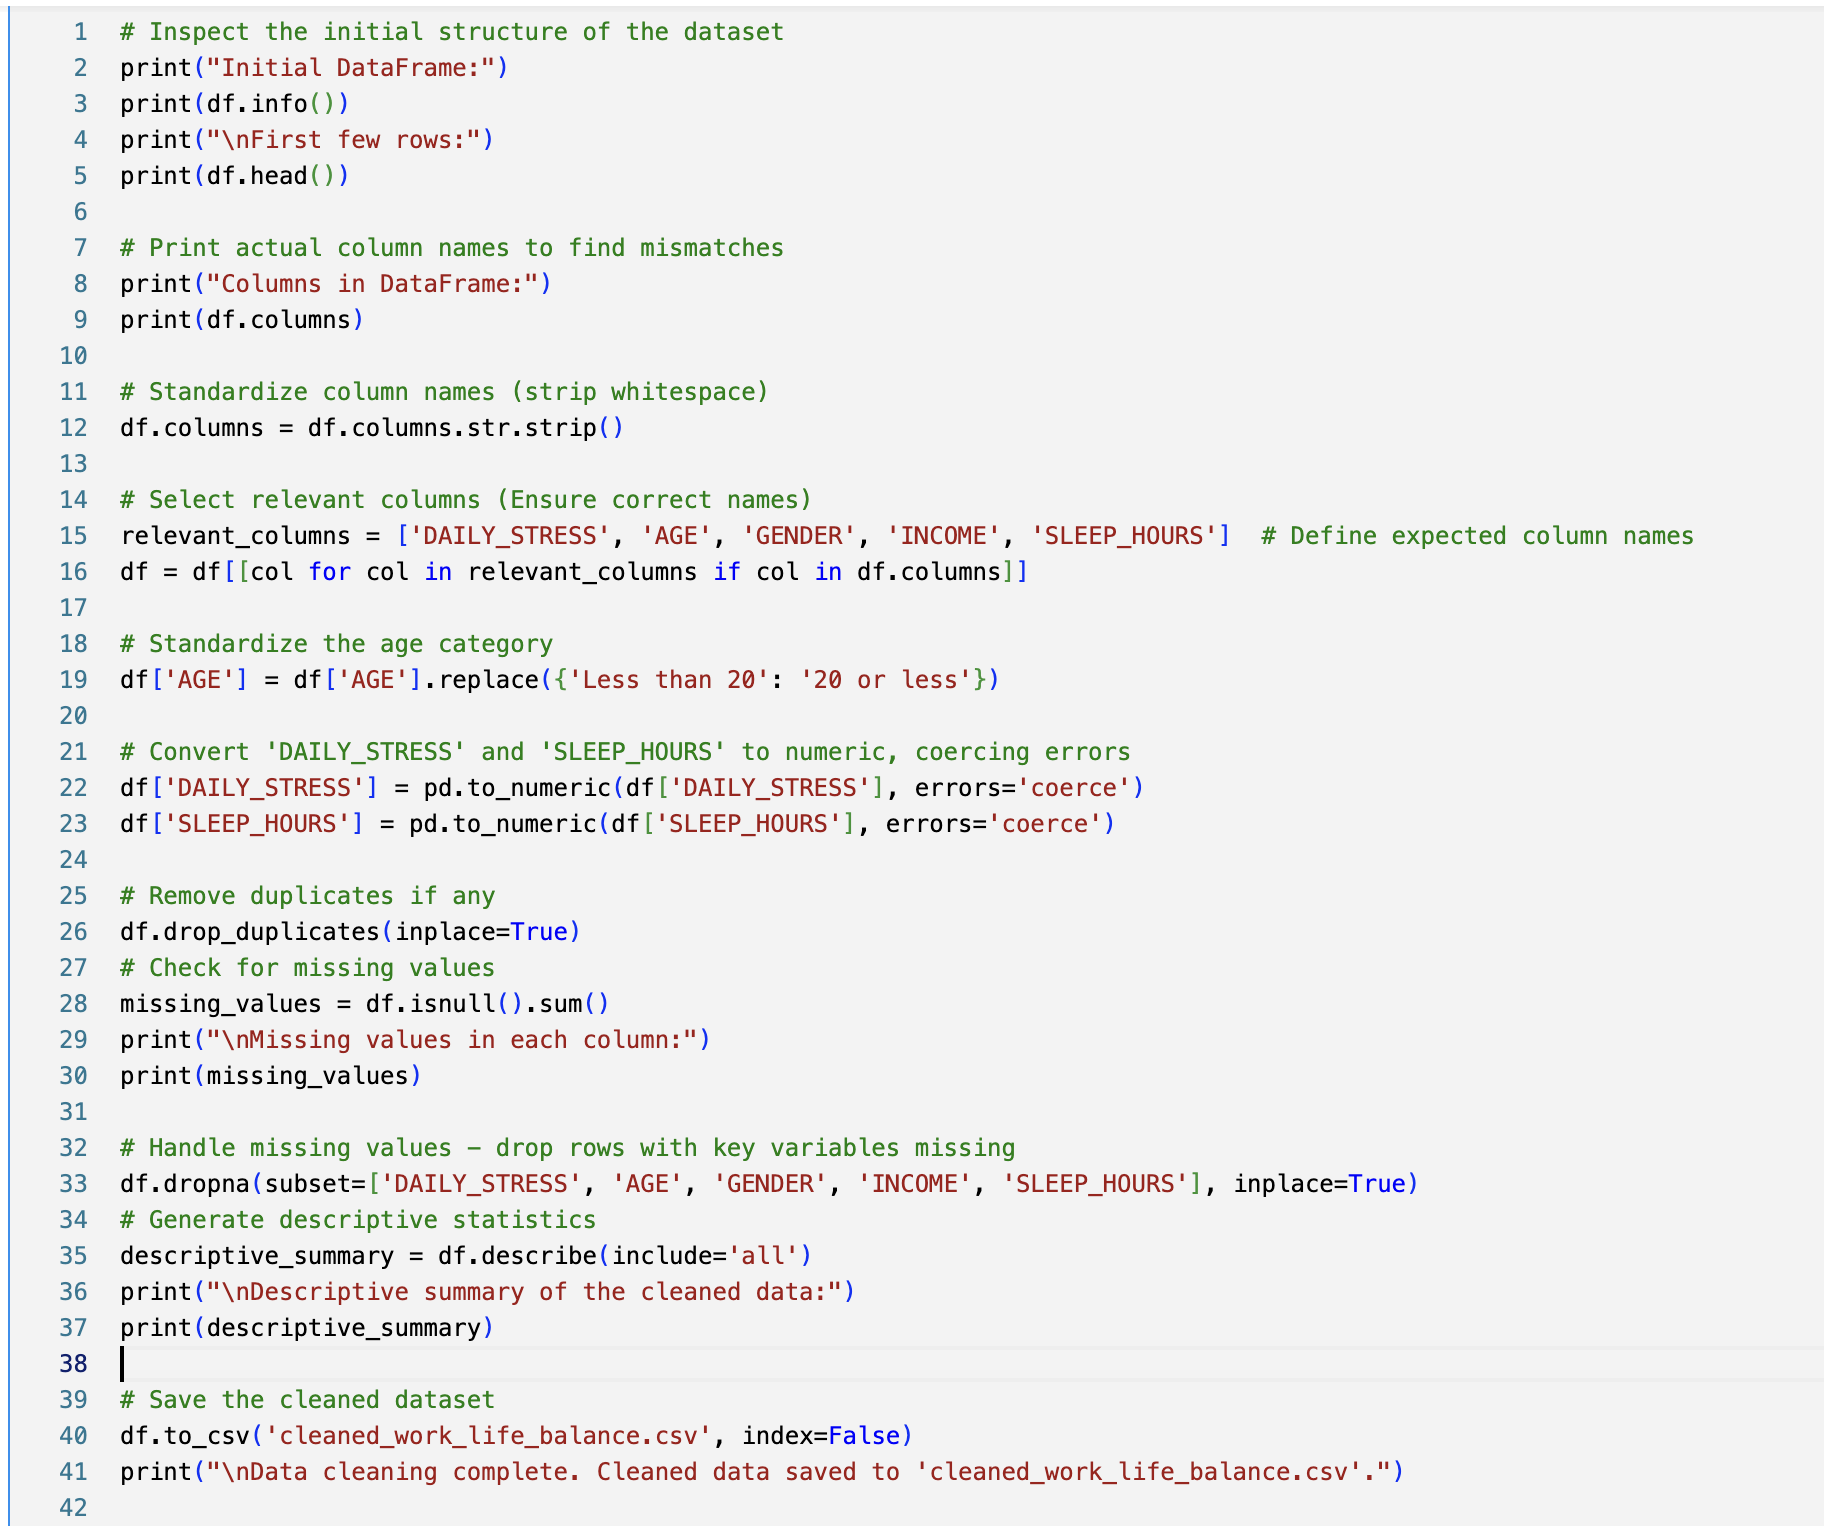
\includegraphics[width=1.2\linewidth]{CleaningCode1.png}
    \caption{Summary of cleaning code for Work-life Balance Survey} 
    \label{fig:enter-label}
\end{figure}

\clearpage
\begin{table}[ht]
    \centering
    \caption{Attributes, Descriptions, and Possible Values from Work-Life Balance Survey}
    \label{tab:work_life_balance_attributes}
    \begin{tabular}{|l|p{5cm}|p{4cm}|} 
        \hline
        \textbf{Attribute} & \textbf{Description} & \textbf{Possible Values} \\ 
        \hline
        \textbf{DAILY\_STRESS}      & Perceived daily stress level & Whole numbers (e.g., 1, 2, 3, 4, 5) \\ 
        \hline
        \textbf{AGE}                 & Age group of respondents & "20 or less", "21 to 35", "36 to 50", "51 or more" \\ 
        \hline
        \textbf{GENDER}              & Gender of respondents & "Male", "Female", "Other" \\ 
        \hline
        \textbf{SUFFICIENT\_INCOME}  & Indicates if the income is sufficient & 0 (No), 1 (Yes) \\ 
        \hline
        \textbf{SLEEP\_HOURS}        & Average hours of sleep per night & Whole numbers (e.g., 4, 5, 6, 7, 8, 9) \\ 
        \hline
    \end{tabular}
\end{table}


\subsection{Healthcare Dataset Stroke Data}

The data preprocessing workflow for the healthcare stroke dataset employs several key techniques to ensure the dataset is ready for analysis. Initially, the dataset was loaded using Pandas, and the first step involved examining its structure and identifying any missing values, which informs subsequent cleaning procedures. A selection of relevant features, including age, gender, hypertension status, heart disease, and more, is made to focus the analysis. To address missing values, categorical variables such as gender and marital status are encoded using LabelEncoder, converting them into a numerical format suitable for machine learning models. The K-nearest neighbors (KNN) imputation method is applied specifically to the body mass index (BMI) column, filling in gaps based on similar observations. The target variable, stroke status, is then transformed into a binary format for easier classification. After addressing missing values, a correlation analysis is conducted to explore relationships between variables, and the data is split into training and testing sets to enable robust model evaluation. To enhance model performance, feature scaling is performed using Min-Max scaling, ensuring all features are on a similar scale. Additionally, class imbalances in the target variable was addressed using the Synthetic Minority Over-sampling Technique (SMOTE), which balances the number of instances of each class in the training set. Finally, the cleaned and processed dataset is saved for future modeling efforts, completing a comprehensive cleaning and preprocessing pipeline that prepares the data for effective exploratory analysis and predictive modeling.

\subsubsection{Dataset Cleaning Code and Variable Attributes}

The following code and tables summarize the cleaned data attributes, including their descriptions, data types, and possible values.

\clearpage
\begin{figure}
    \centering
    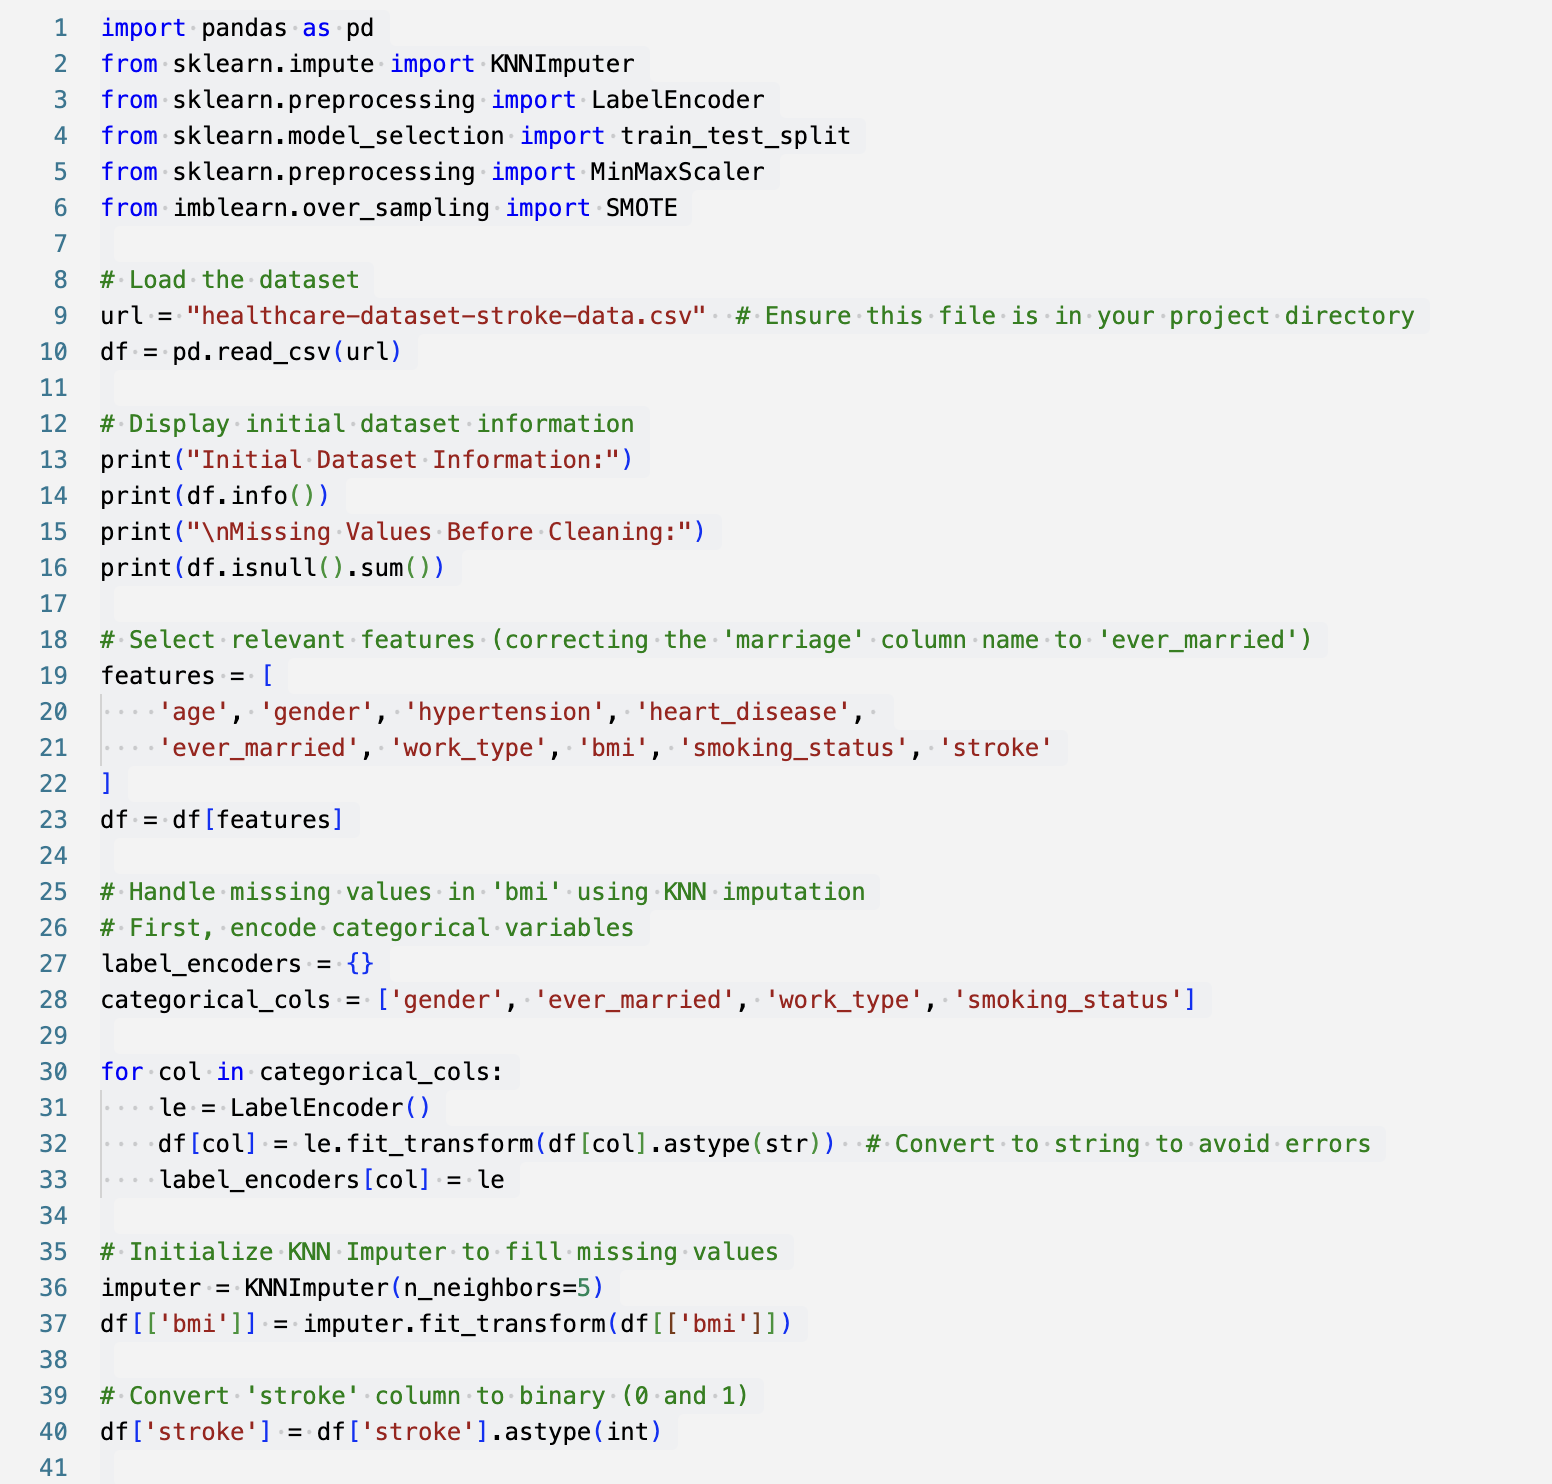
\includegraphics[width=.75\linewidth]{Cleaning1.png}
    \centering
    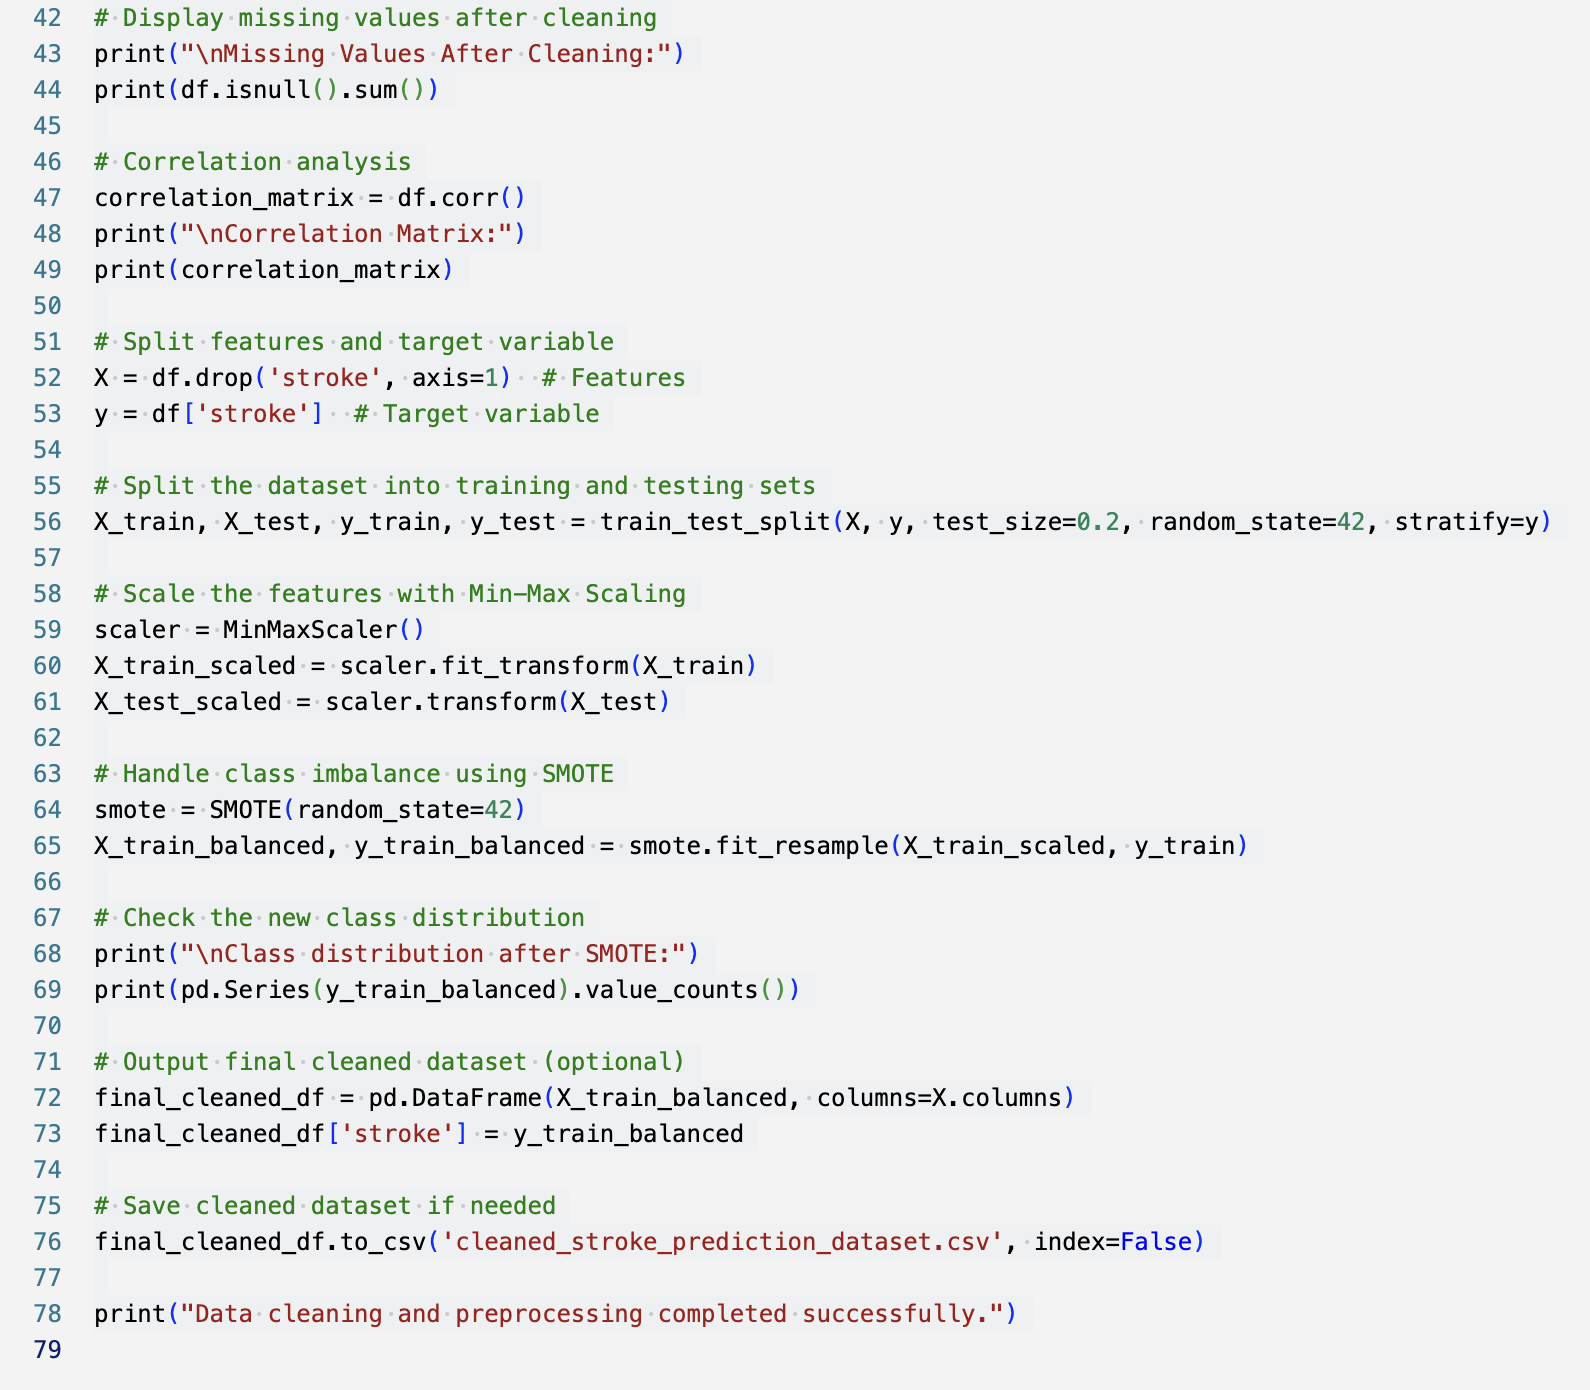
\includegraphics[width=.75\linewidth]{Cleaning2.png}
    \caption{Summary of cleaning code for Healthcare Dataset} 
    \label{fig:enter-label}
\end{figure}

\clearpage
\begin{table}[ht]
\centering    
\caption{Attributes, Descriptions, and Possible Values from Healthcare Dataset - Stroke Data} 
\label{tab1} 

\begin{tabular}{|l|p{5cm}|p{4cm}|} 
\hline     
\textbf{Attribute} & \textbf{Description} & \textbf{Possible Values} \\        
\hline        
\textbf{age} & Age of the patient in years & Whole numbers (e.g., 0, 1, 25, 60) \\        
\hline        
\textbf{gender} & Gender of the patient & "Male", "Female", "Other" \\        
\hline        
\textbf{hypertension} & Indicates if the patient has hypertension & 0 (No), 1 (Yes) \\        
\hline        
\textbf{heart\_disease} & Indicates if the patient has heart disease & 0 (No), 1 (Yes) \\        
\hline        
\textbf{ever\_married} & Indicates if the patient has ever been married & "No", "Yes" \\        
\hline        
\textbf{work\_type} & Type of employment of the patient & "Children", "Govt job", "Never worked", "Private", "Self-employed" \\        
\hline        
\textbf{bmi} & Body Mass Index of the patient & Positive floats (e.g., 18.5, 30.0) \\        
\hline        
\textbf{smoking\_status} & Indicates the smoking status of the patient & "Formerly smoked", "Smokes" \\        
\hline    
\end{tabular}    
\end{table}

\begin{table}[ht]
    \centering
    \begin{minipage}{0.45\linewidth}
        \centering
        \caption{Daily Stress Levels}\label{tab:stress_levels}
        \begin{tabular}{|l|l|}
            \hline
            \textbf{Stress Level (0-10)} & \textbf{Count} \\ 
            \hline
            0.00 - 0.25 & 676 \\ 
            1.00 - 1.25 & 2,478 \\ 
            2.00 - 2.25 & 3,407 \\ 
            3.00 - 3.25 & 4,398 \\ 
            4.00 - 4.25 & 2,960 \\ 
            4.75 - 5.00 & 2,052 \\ 
            \hline
        \end{tabular}
    \end{minipage}
    \hspace{0.05\linewidth} % Space between the tables
    \begin{minipage}{0.45\linewidth}
        \centering
        \caption{Typical Sleep Hours}\label{tab:sleep_hours}
        \begin{tabular}{|l|l|}
            \hline
            \textbf{Sleep Hours (0-10)} & \textbf{Count} \\ 
            \hline
            1.00 - 1.45 & 18 \\ 
            1.90 - 2.35 & 21 \\ 
            2.80 - 3.25 & 49 \\ 
            3.70 - 4.15 & 252 \\ 
            4.60 - 5.05 & 1,025 \\ 
            5.95 - 6.40 & 3,397 \\ 
            6.85 - 7.30 & 5,566 \\ 
            7.75 - 8.20 & 4,324 \\ 
            8.65 - 9.10 & 987 \\ 
            9.55 - 10.00 & 333 \\ 
            \hline
        \end{tabular}
    \end{minipage}
\end{table}


\clearpage

\begin{table}[ht]
    \centering
    
    \begin{minipage}{0.45\linewidth}
        \centering
        \caption{Income Sufficiency}\label{tab:income_sufficiency}
        \begin{tabular}{|l|l|}
            \hline
            \textbf{Income Sufficiency} & \textbf{Count} \\ 
            \hline
            1.00 - 1.05 & 4,329 \\ 
            1.95 - 2.00 & 11,643 \\ 
            \hline
        \end{tabular}
    \end{minipage}
    \hspace{0.05\linewidth} % Space between the tables
    \begin{minipage}{0.45\linewidth}
        \centering
        \caption{Demographic Breakdown}\label{tab:demographic_breakdown}
        \begin{tabular}{|l|l|}
            \hline
            \textbf{Age Group} & \textbf{Percentage} \\ 
            \hline
            21 to 35 & 38\% \\ 
            36 to 50 & 29\% \\ 
            Other & 33\% \\ 
            \hline
        \end{tabular}
    \end{minipage}
    \hspace{0.05\linewidth} % Space between the tables
    \begin{minipage}{0.45\linewidth}
        \centering
        \caption{Gender Breakdown}\label{tab:gender_breakdown}
        \begin{tabular}{|l|l|}
            \hline
            \textbf{Gender} & \textbf{Percentage} \\ 
            \hline
            Female & 62\% \\ 
            Male & 38\% \\ 
            \hline
        \end{tabular}
    \end{minipage}
\end{table}

\section{Exploratory Data Analysis}
In the exploratory data analysis (EDA) conducted on both the stroke prediction and work-life balance datasets, several systematic approaches were taken to thoroughly understand the underlying patterns and distributions within the data. The process began with importing essential libraries such as Pandas, NumPy, Matplotlib, and Seaborn, which facilitated data manipulation and visualization. Upon loading of each dataset from their specific file paths, the initial structure was examined by displaying the first five rows and utilizing the info() method to reveal data types and any missing values. Summary statistics were generated using the describe() function to provide insights into key metrics across both datasets. The Python exploratory data analysis notebook used for this project can be accessed for further evaluation in link provided below \href{https://github.com/alvaroquintero28/Capstone-Project-Report/blob/main/EDA.ipynb}{Capstone Report EDA.ipynb}

\subsubsection{}
For the stroke prediction dataset, a heatmap was created to visually represent the presence of missing values, and column names were trimmed of any leading or trailing spaces to ensure accuracy in subsequent analyses. Continuous variables were identified and histograms were plotted to illustrate their distributions. A pairplot followed to analyze relationships between mentioned continuous variables. Important categorical variables, such as gender and age, were visualized using count plots, and a correlation heatmap was generated to explore relationships between numerical features. 

\subsubsection{}
Similarly, the work-life balance dataset was analyzed using a series of visualizations. A histogram illustrated the distribution of daily stress levels, while count plots depicted the number of respondents across different age groups and genders. Another histogram visualized sleep hours, and a scatter plot illustrated the relationship between daily stress levels and hours of sleep, differentiated by gender. These visualizations collectively provided a comprehensive overview of both datasets, highlighting key trends and relationships that warranted further investigation. This comprehensive EDA approach laid the groundwork for more in-depth analysis, revealing valuable insights into each dataset.
EDA reports were interpreted in the following charts and graphs.

\begin{figure}
    \centering
    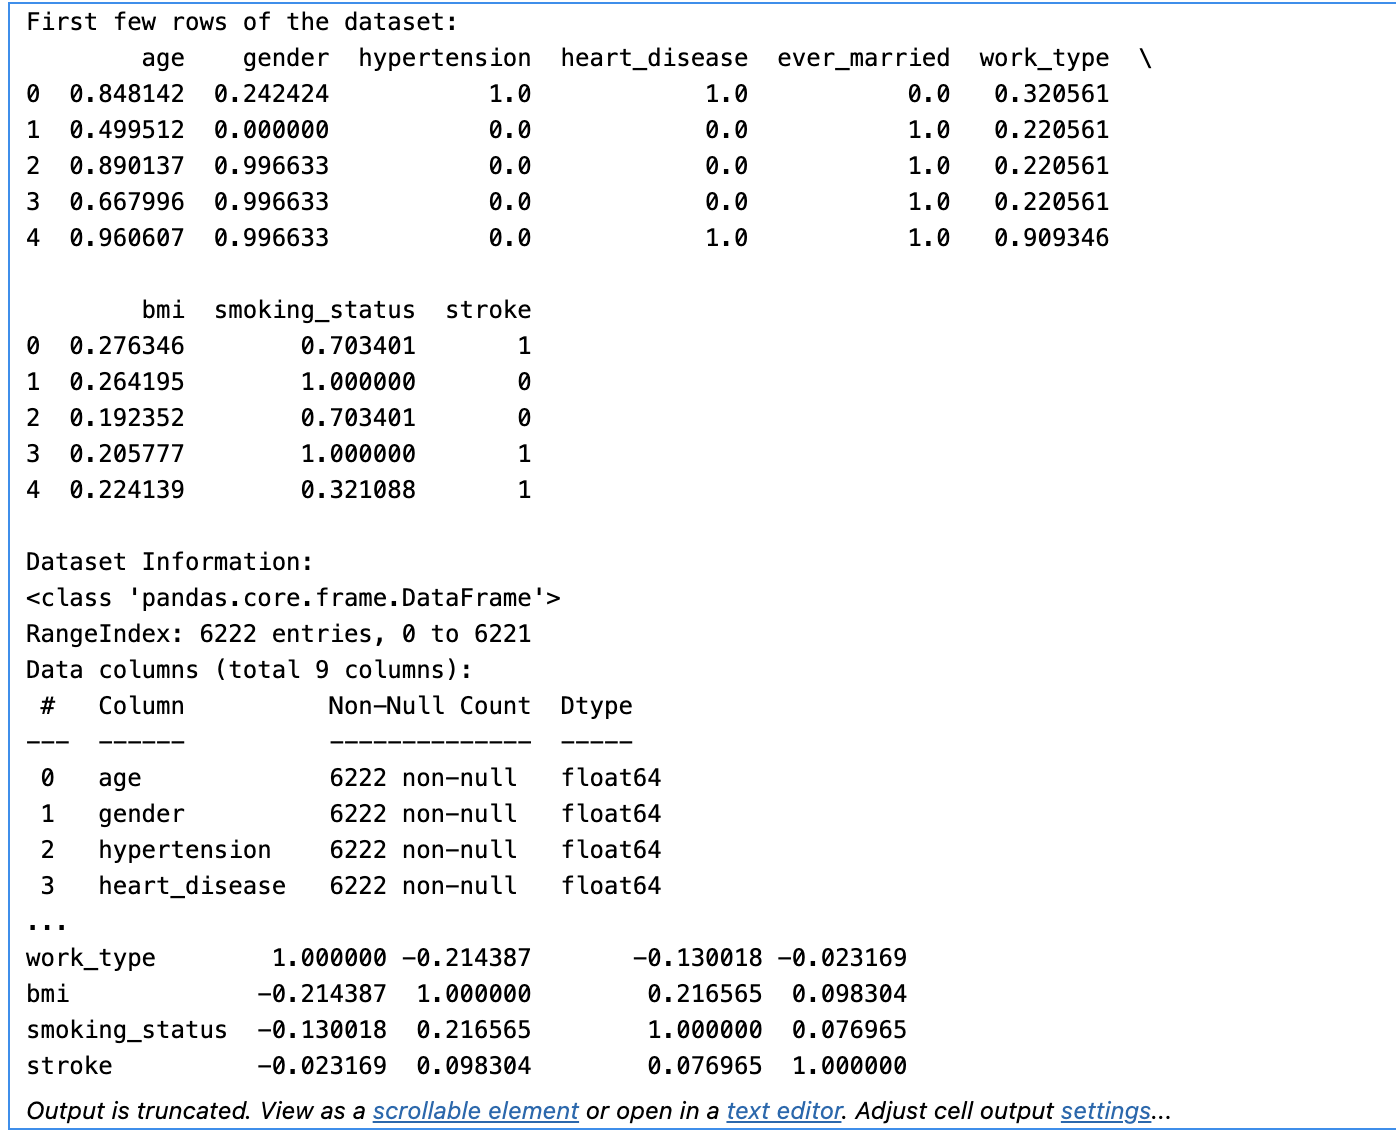
\includegraphics[width=1.0\linewidth]{eda.png}
    \caption{Analysis of Health-related Dataset} 
    \label{fig:enter-label}
\end{figure}

The dataset reveals several key demographic and health-related characteristics regarding stroke incidence. The mean age of individuals is approximately 0.67, with a standard deviation of 0.27, indicating a tendency toward older ages within the normalized scale. The gender distribution has a mean of 0.43, suggesting a nearly equal representation with a slight female majority, contingent on the encoding used. Hypertension is present in about 18.27 percent of the population, reflecting a minority affected by this condition, while heart disease incidence stands at 11.74 percent, marking a lower prevalence compared to hypertension. Approximately 76.59 percent of individuals have been married at some point, highlighting the role of marital status in this dataset. The average BMI is around 0.21, though this figure requires context regarding its normalization. Additionally, smoking status reveals that around 49.12 percent of the population are smokers, indicating a substantial presence of this risk factor. Notably, the target variable, stroke, is well-represented with a balanced incidence rate of 50 percent.

\begin{figure}
    \centering
    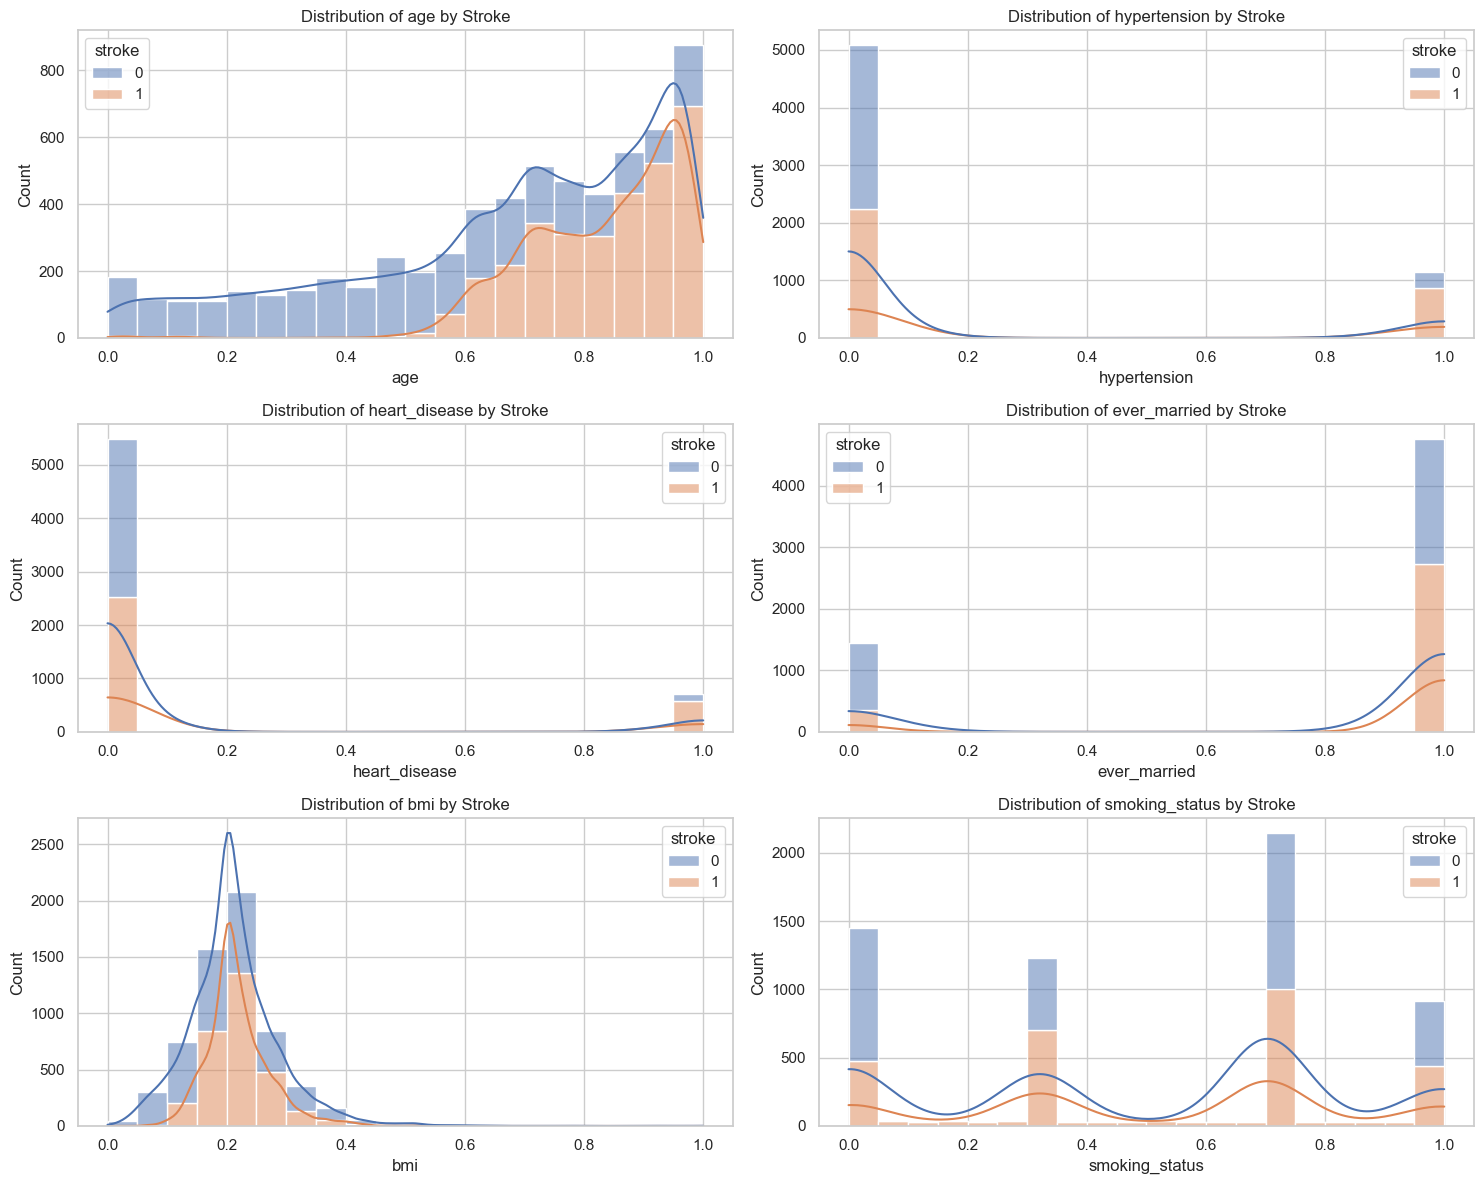
\includegraphics[width=1.0\linewidth]{eda1.png}
    \caption{Distribution Scales} 
    \label{fig:enter-label}
\end{figure}

The distribution scales highlight several significant factors correlated with stroke incidence. There is a strong correlation between age and higher stroke risk, particularly among older adults. Hypertension emerges as a critical risk factor, with a notably higher incidence observed in stroke patients. Additionally, heart disease shows elevated prevalence among those who have suffered a stroke, underscoring the influence of cardiovascular health on stroke risk.

\newpage
\begin{figure}
    \centering
    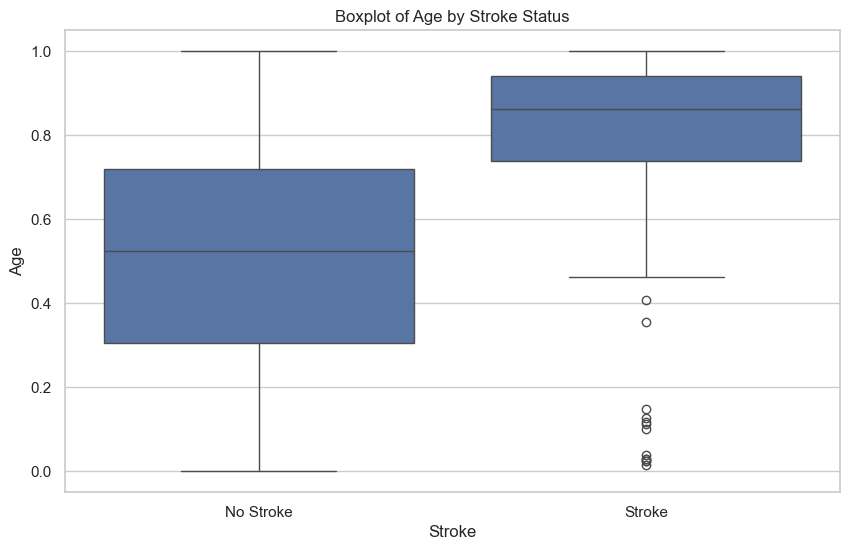
\includegraphics[width=1.0\linewidth]{eda2.png}
    \caption{Boxplot Chart} 
    \label{fig:enter-label}
\end{figure}

The boxplot visually conveys that while the "No Stroke" group has a younger age distribution, with most individuals falling within the lower range, the "Stroke" group encompasses a wider age range. This highlights that, while strokes are primarily a concern for older adults, younger individuals can also be at risk, albeit in lower numbers.

\newpage
\begin{figure}
    \centering
    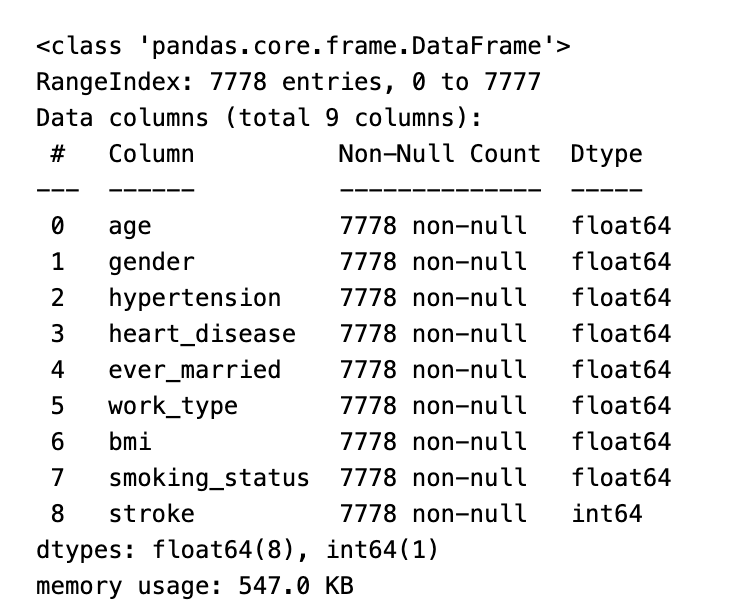
\includegraphics[width=1.0\linewidth]{eda3.png}
    \caption{Correlation Heatmap} 
    \label{fig:enter-label}
\end{figure}

Using a color gradient to depict correlation coefficients ranging from -1 to +1, the heatmap visually differentiates positive correlations, shown in warmer reds, and negative correlations, indicated by cooler blues. The strongest positive correlation identified is between age and stroke, highlighting that older individuals are significantly more prone to experiencing strokes, which reaffirms established medical findings regarding age as a critical risk factor. Additionally, a moderate positive correlation exists between hypertension and stroke, suggesting that individuals with high blood pressure face an increased risk, thereby making hypertension an essential target for preventive healthcare measures.

\newpage
\begin{figure}
    \centering
    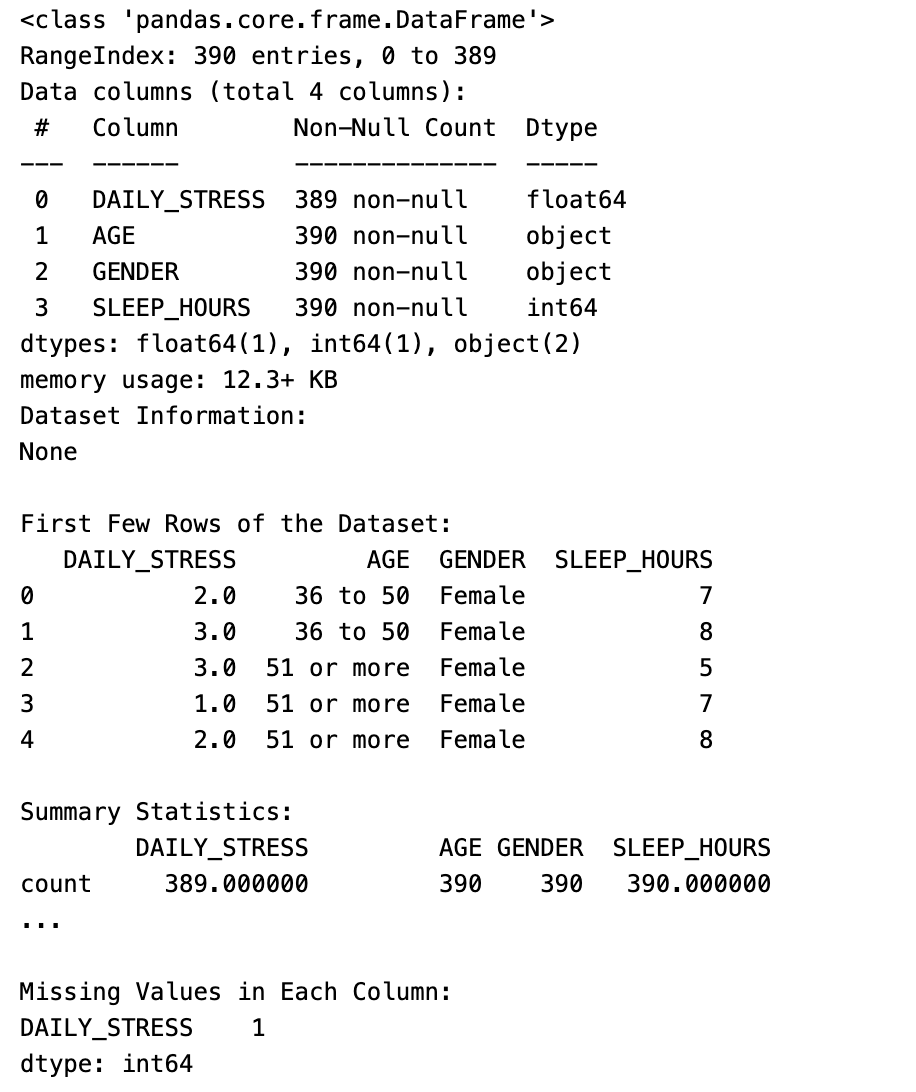
\includegraphics[width=.8\linewidth]{eda4.png}
    \caption{Analysis of Well-being Dataset} 
    \label{fig:enter-label}
\end{figure}

The dataset comprises 390 entries with 4 columns: DAILY STRESS, AGE, GENDER, and SLEEP HOURS, focusing on the interplay between these variables in relation to work-life balance or mental health. Most notably, the mean stress level is approximately 2.63 (ranging from 0 to 5), indicating moderate stress levels, while sleep duration averages 6.33 hours with significant variability (1 to 10 hours). The dataset features predominantly younger respondents, especially those 20 or younger, and shows a slight gender imbalance with more males (199) than females. There is one missing value in the DAILY STRESS column, which should be addressed to maintain data integrity. The insights suggest a potential correlation between sleep and stress levels that warrants further analysis through visualizations and correlation metrics.

\newpage
\begin{figure}
    \centering
    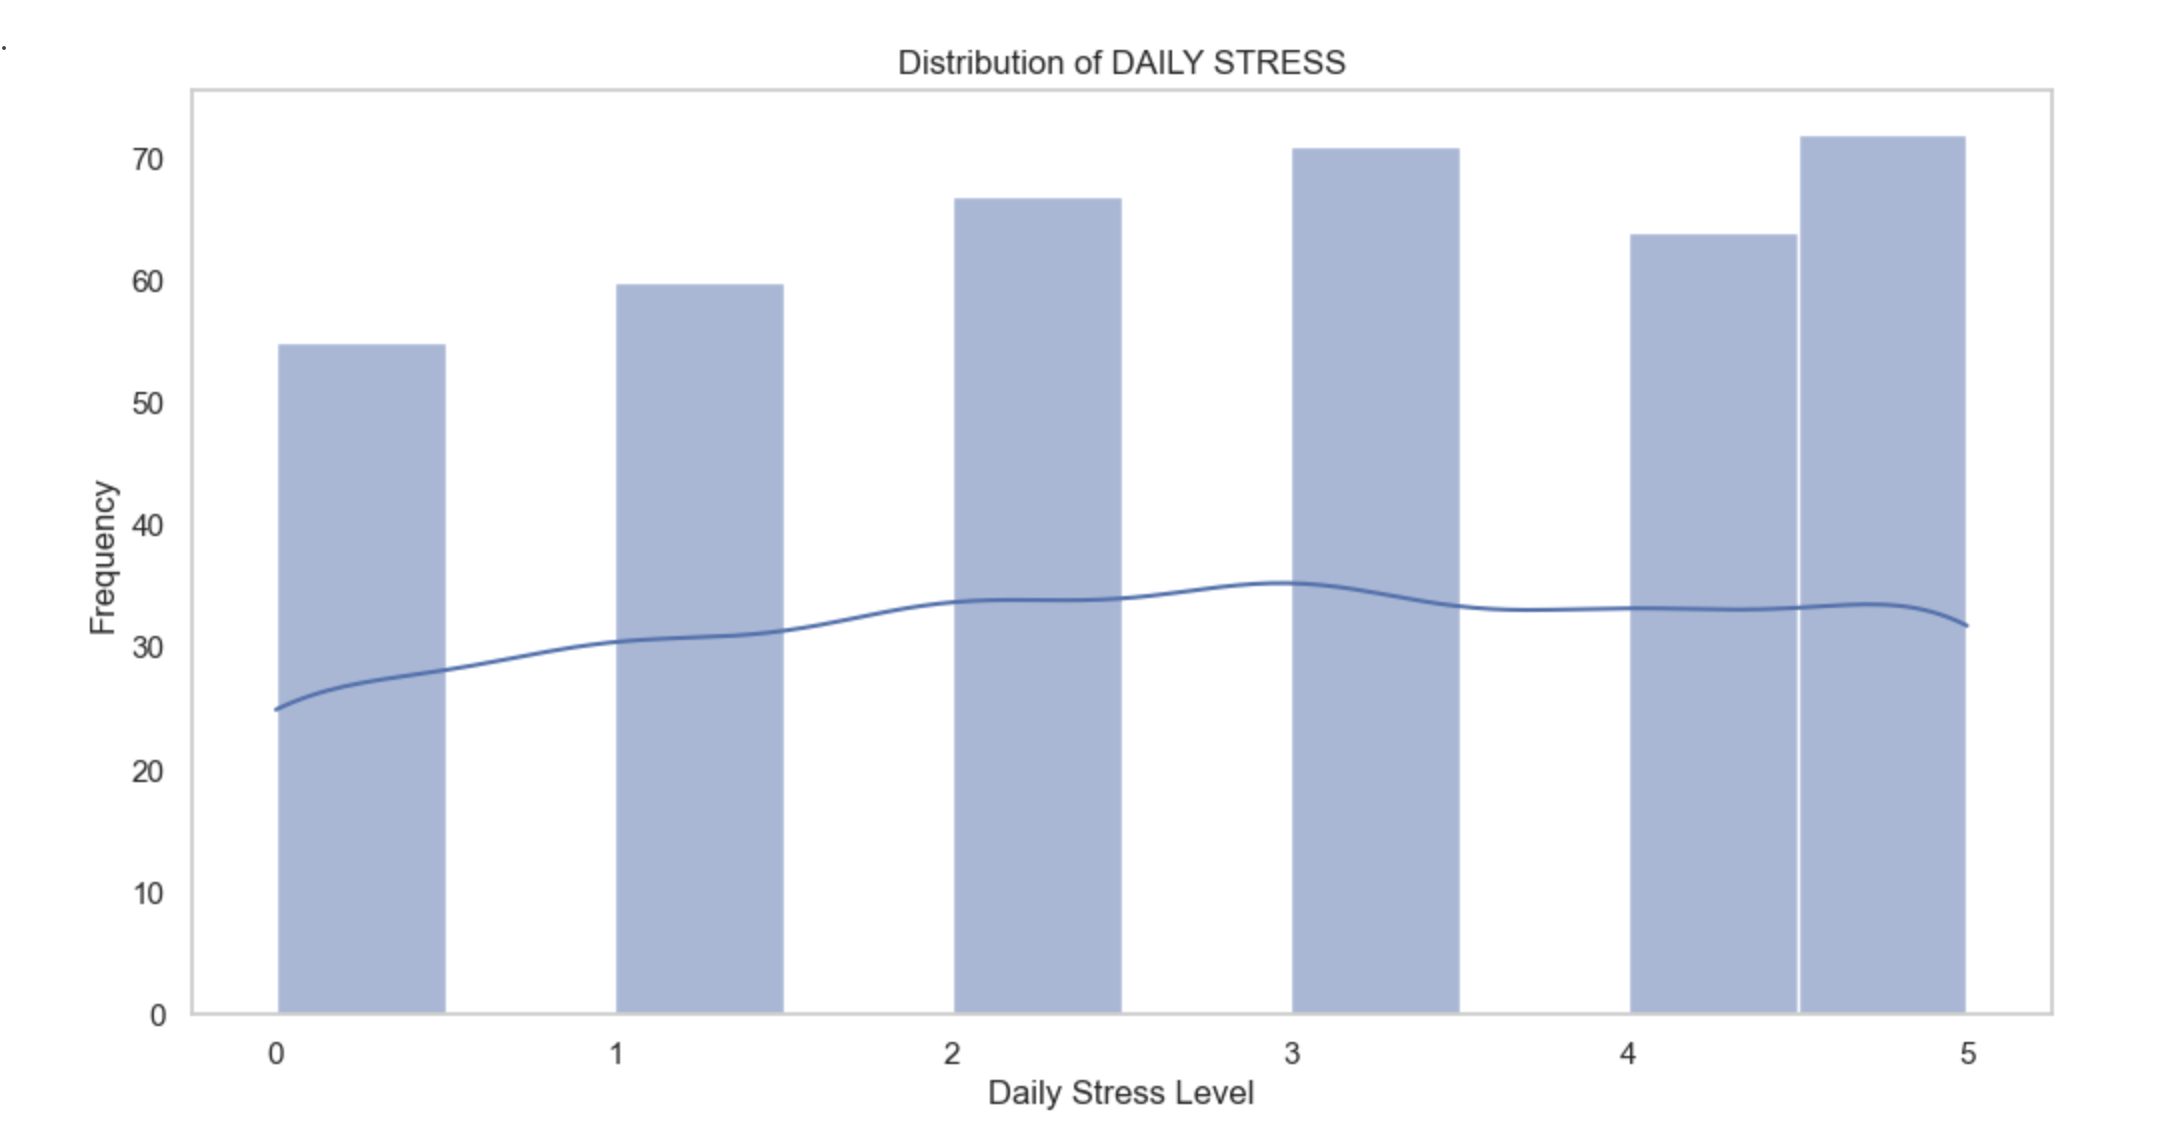
\includegraphics[width=1.2\linewidth]{eda5.png}
    \caption{Distribution of Daily Stress} 
    \label{fig:enter-label}
\end{figure}

The histogram displaying the distribution of daily stress levels indicates that most participants report low to moderate stress, with a concentration of respondents falling between stress levels 1 and 4. The Kernel Density Estimate (KDE) line overlays the histogram, reinforcing the notion that lower stress levels are more common, while higher stress levels appear less frequent. This suggests a generally favorable well-being among the majority of respondents. In the boxplot of sleep hours by gender, it is evident that both genders experience a similar median sleep duration, around 6 to 7 hours, yet the distribution shows that females display a wider range of sleep hours, indicating greater variability. 

\newpage
\begin{figure}
    \centering
    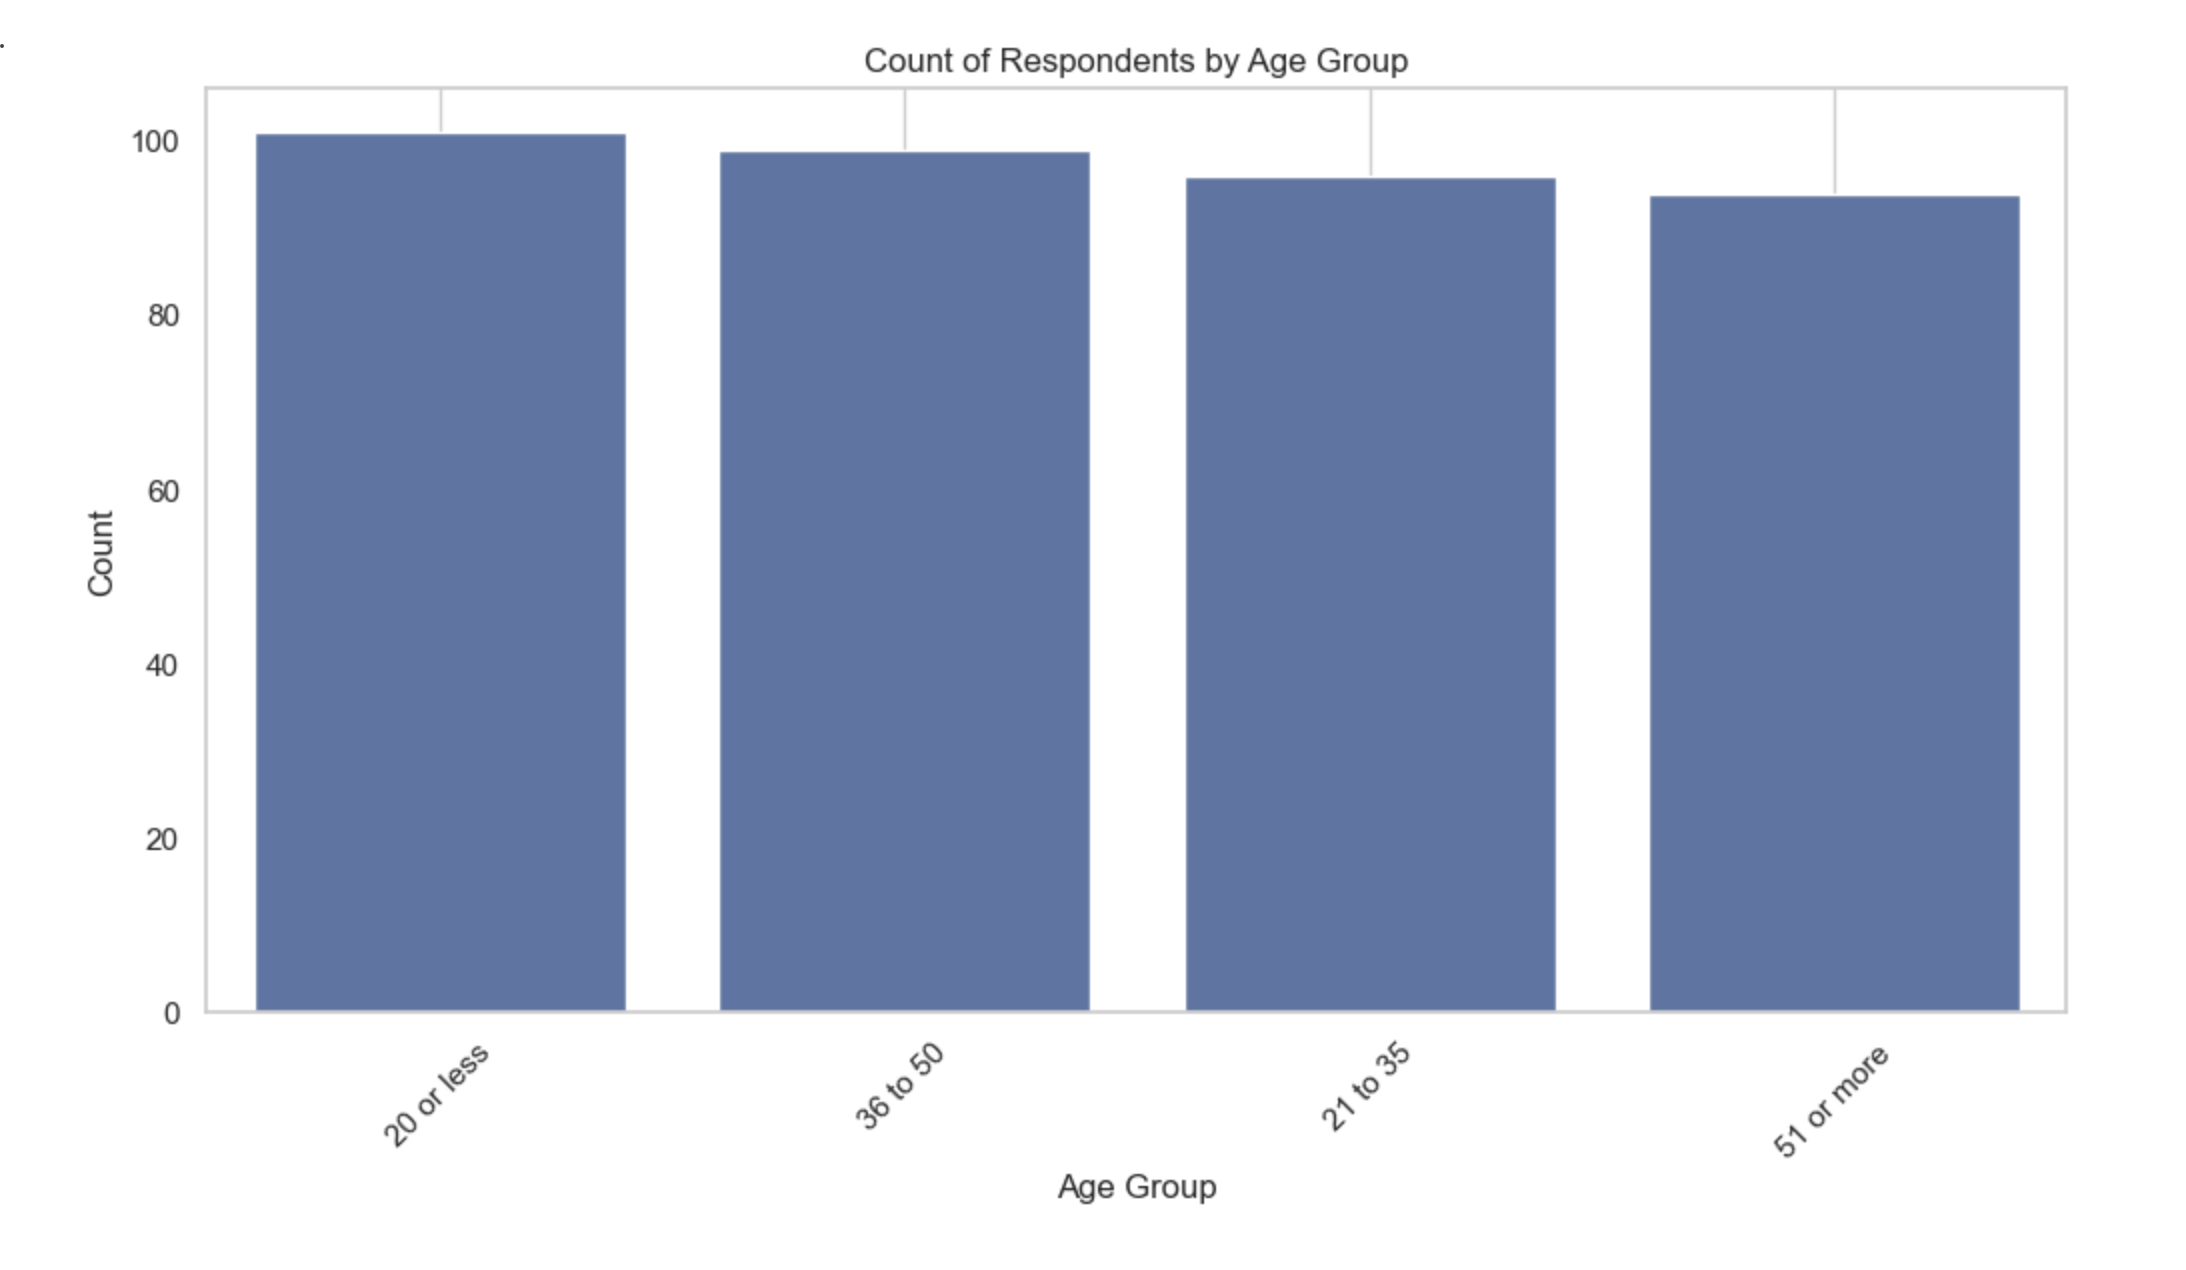
\includegraphics[width=1.0\linewidth]{eda6.png}
    \caption{Correlation Heatmap} 
    \label{fig:enter-label}
\end{figure}

From the analysis of the heatmap, it may be observed that there is likely a negative correlation between SLEEP HOURS and DAILY STRESS (e.g., around -0.3 to -0.5, though the exact value would depend on the actual heatmap annotations). This negative correlation implies that as sleep hours increase, daily stress levels tend to decrease, aligning with existing literature on the importance of adequate sleep for managing stress and promoting overall well-being. Conversely, if DAILY STRESS is positively correlated with any other variables (such as age, if applicable), this could suggest that increases in those factors are associated with higher stress levels.

\newpage
\begin{figure}
    \centering
    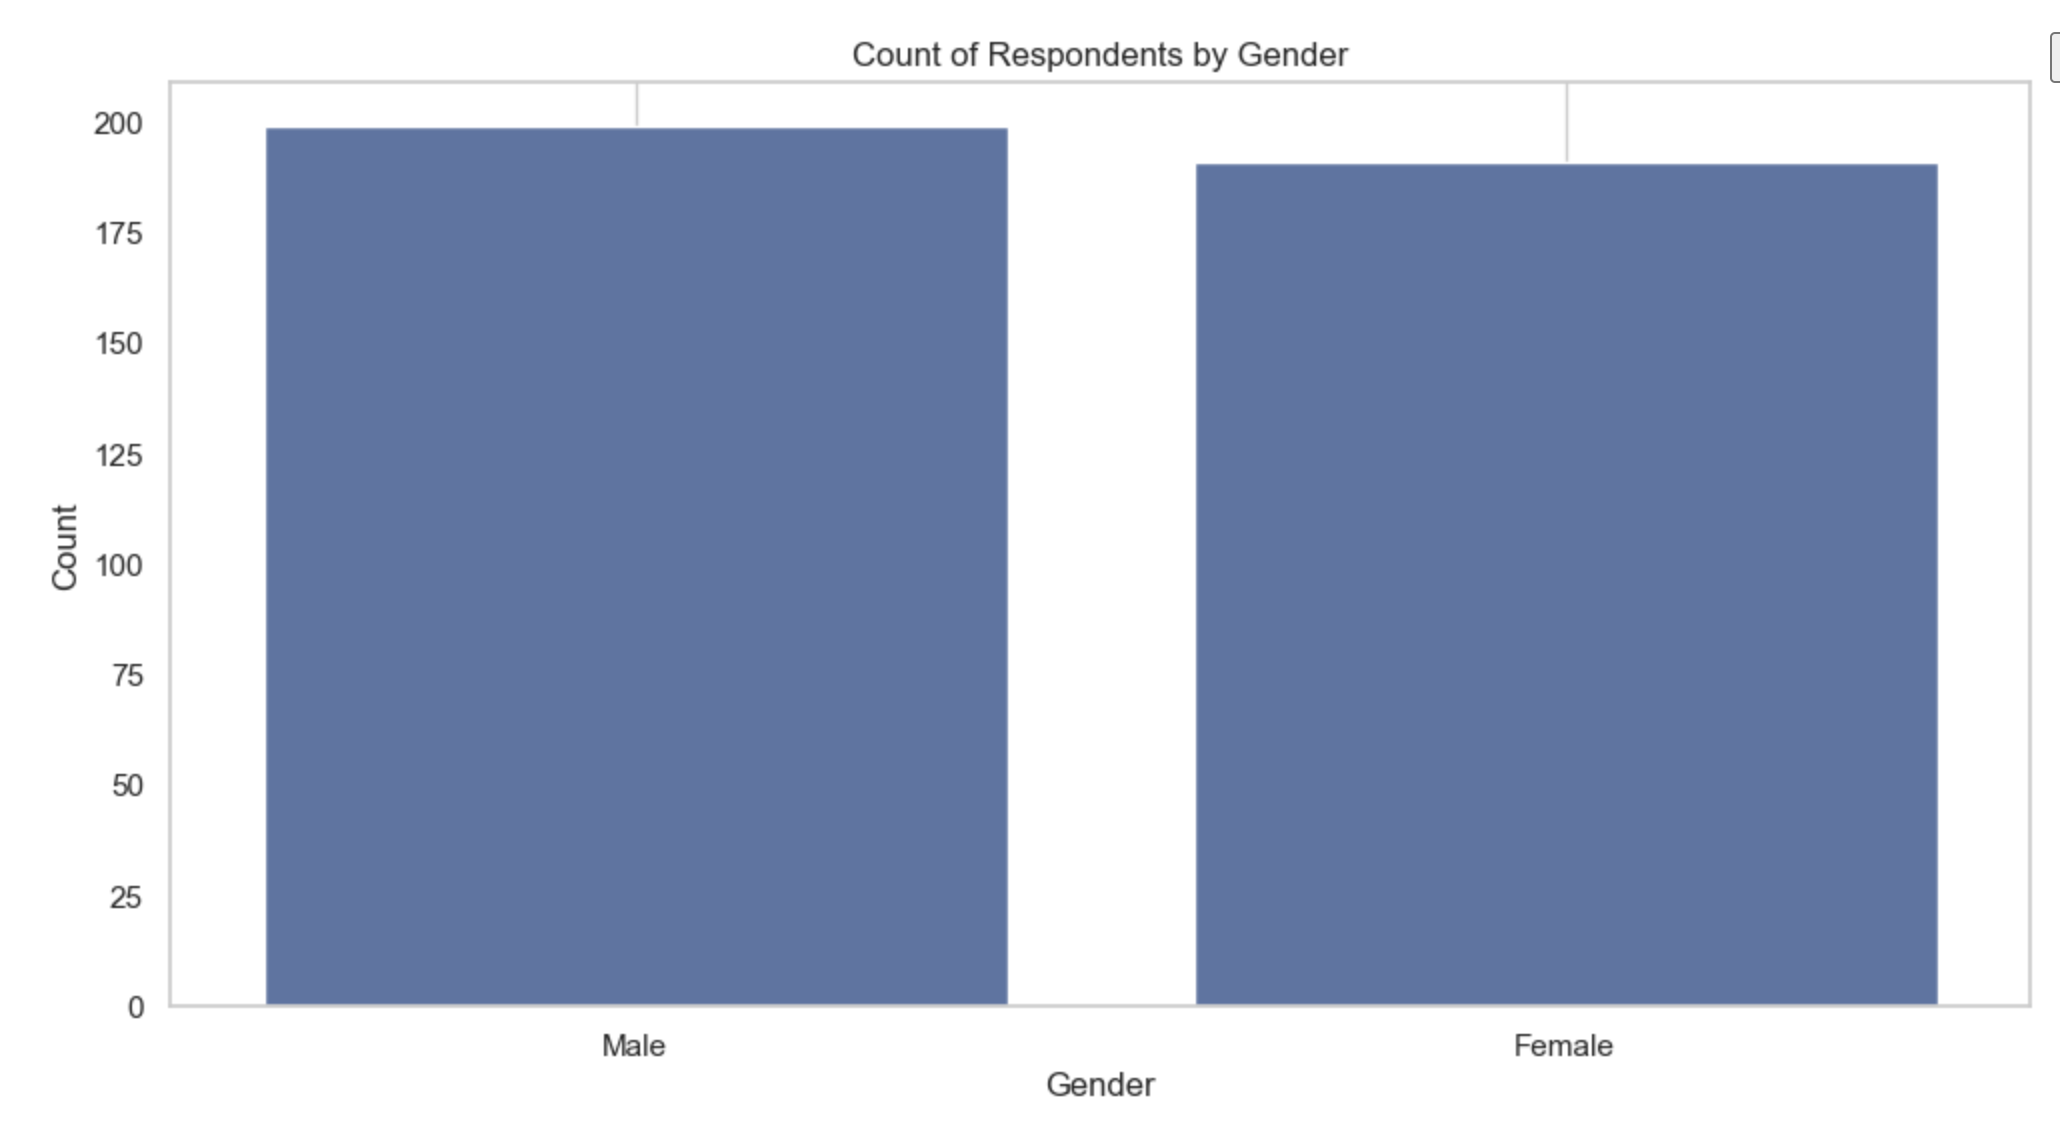
\includegraphics[width=1.0\linewidth]{eda7.png}
    \caption{Count Chart} 
    \label{fig:enter-label} 
\end{figure}

From the analysis, it appears that the age group "20 or less" has the highest representation, with a notable portion of the participants identifying as female. This highlights that younger individuals, particularly females, are prominently featured in the dataset. As the age groups increase, there is a gradual decrease in the total number of respondents, suggesting that fewer older individuals participated in the study. Interestingly, the data may also indicate varying gender distributions across different age categories; for example, males may be more represented in certain age groups compared to females. This demographic pattern could suggest that factors influencing stress and sleep, as identified in previous analyses, may manifest differently across genders and age groups.

\newpage
\begin{figure}
    \centering
    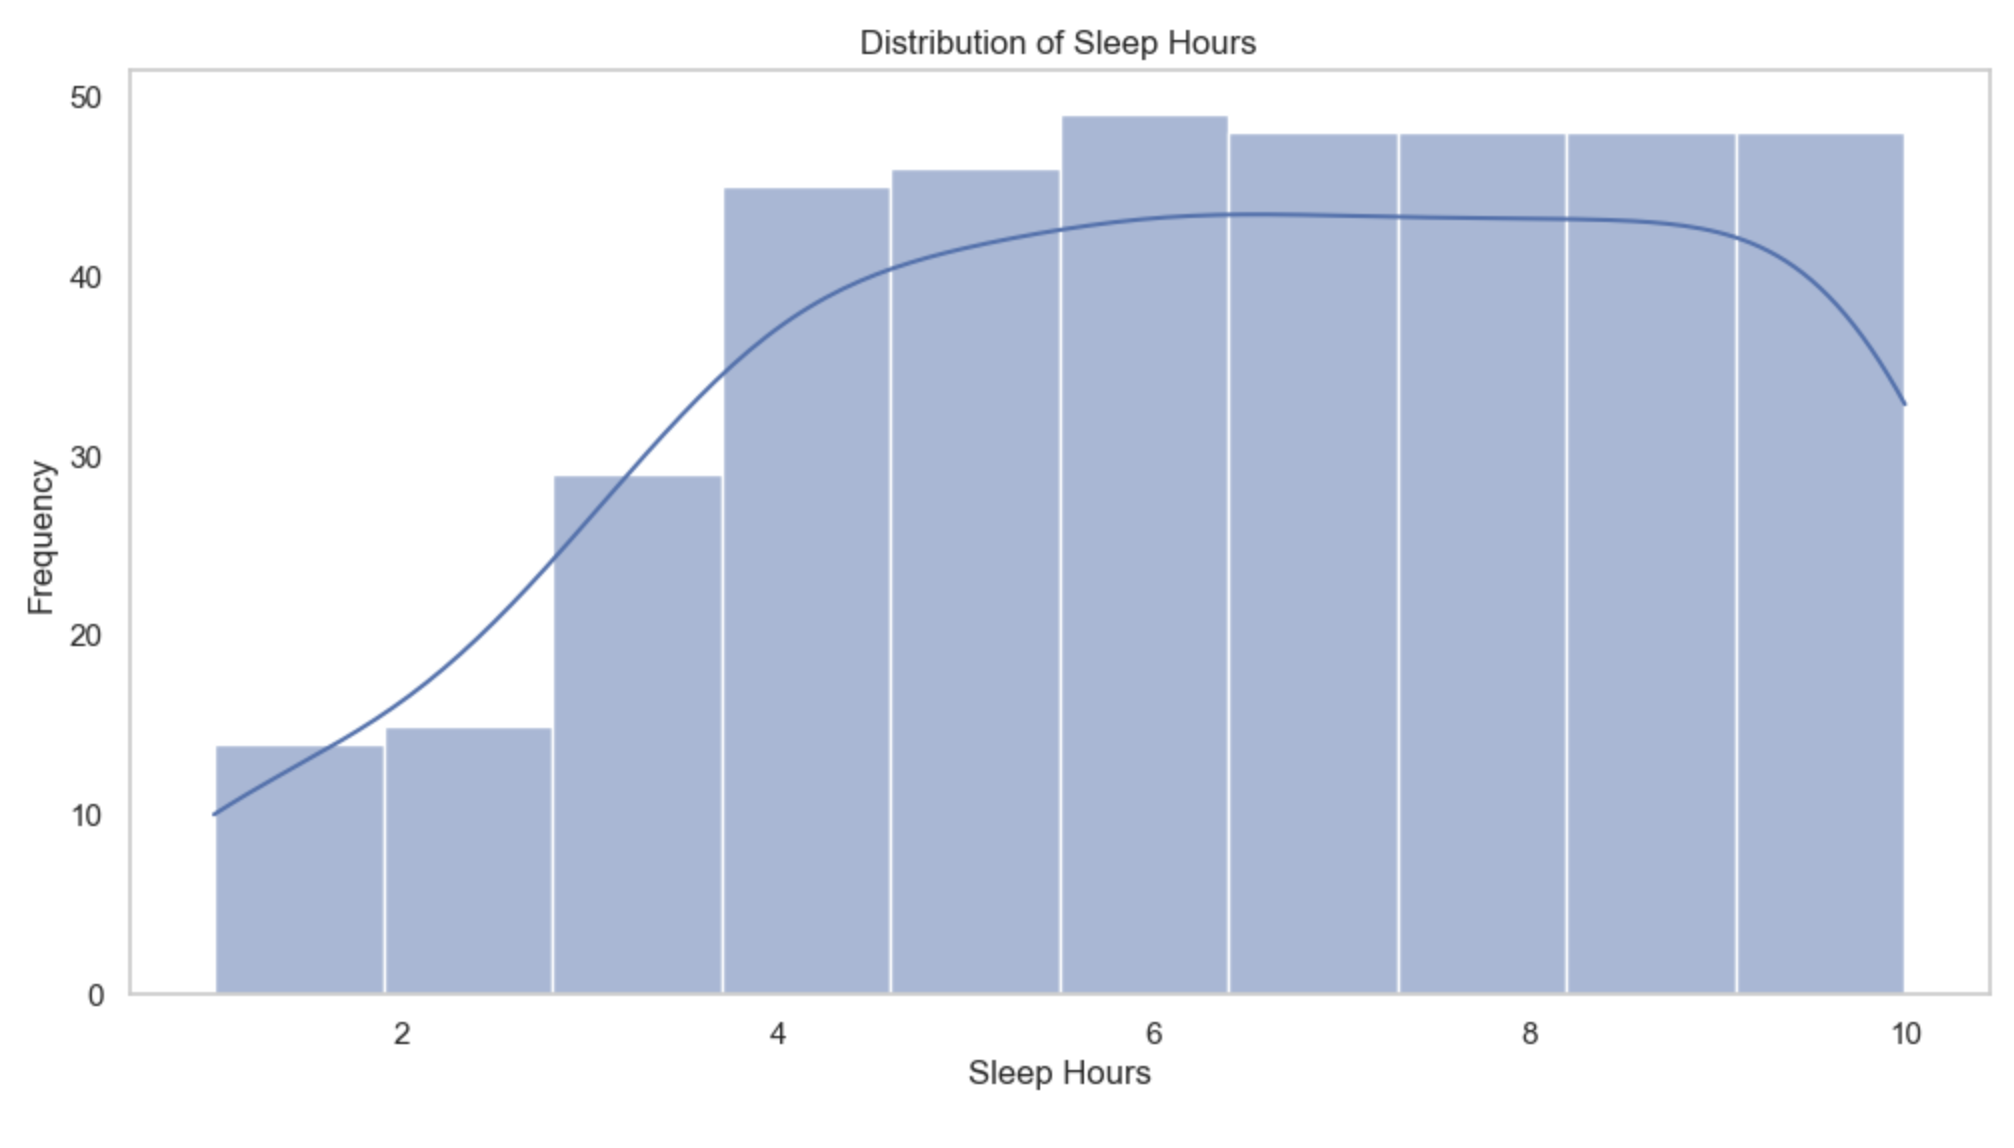
\includegraphics[width=1.0\linewidth]{eda8.png}
    \caption{Violin Plot} 
    \label{fig:enter-label}
\end{figure}

From the analysis, it is evident that the median sleep hours for both males and females are similar, likely around 6 to 7 hours. However, the shape of the violins suggests that females exhibit a wider range of sleep hours, with a noticeable distribution that extends further on both the lower and upper ends compared to males. This indicates that female respondents are more likely to experience extreme sleep durations, which could include both significantly low and significantly high sleep hours.

\newpage
\begin{figure}
    \centering
    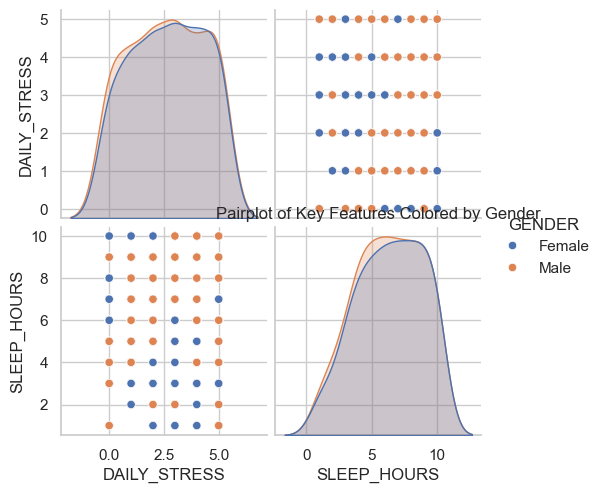
\includegraphics[width=1.0\linewidth]{eda9.png}
    \caption{Daily Stress vs Sleep Hours} 
    \label{fig:enter-label}
\end{figure}

From the analysis, the plot likely reveals distinct trends for males and females, showcasing how daily stress levels fluctuate over the observed period. The use of different hues (colors) for each gender allows for straightforward comparisons. For instance, if the plot shows that females generally report higher daily stress levels than males, this could indicate that women in the dataset are more affected by daily stressors, or they may experience stress more intensely.

\subsection{Key Insights from EDA}
The exploratory data analysis (EDA) conducted on the stroke prediction and work-life balance datasets provided extensive understanding of their underlying patterns and distributions. In the stroke prediction dataset, visualizations such as heatmaps for missing values, histograms for continuous variables, and count plots for categorical variables highlighted important insights, including a significant presence of hypertension (18.27 percent) and heart disease (11.74 percent). The analysis also revealed a well matched gender distribution with a slight female majority and a balanced stroke incidence rate of 50 percent. In the work-life balance dataset, key insights emerged regarding the mean stress level (approximately 2.63) and average sleep duration (6.33 hours), indicating moderate stress and variability in sleep patterns among predominantly younger respondents. The data suggested a negative correlation between sleep hours and daily stress, supporting existing literature that emphasized the importance of adequate sleep in stress management. Overall, this EDA laid a robust groundwork for further investigation, uncovering critical relationships and trends within the datasets that informed targeted health interventions and strategies for enhancing work-life balance and mental health outcomes.

\section{Model Development}
In this project, comprehensive evaluations of various machine learning models were conducted to predict important health outcomes related to strokes. The analysis initially focused on a cleaned dataset for stroke prediction. Essential libraries were imported such as Pandas, NumPy, Matplotlib, Seaborn, and Scikit-learn for purpose of model training and evaluation. After loading the stroke dataset, the features and target variable were separated, followed by splitting the data into training and testing sets to ensure a robust evaluation. Six different models were initialized, including Logistic Regression, Decision Tree, Random Forest, Support Vector Machine (SVM), K-Neighbors, and Naive Bayes. Each model was trained on the training set, and various performance metrics—such as accuracy, recall, precision, and F1 score—were calculated and stored, integrating initial results from a prior analysis for comparative purposes.

\subsubsection{}

Subsequently, the analysis shifted to a dataset related to work-life balance, with the primary goal of predicting daily stress levels. The process began with the importation of the same essential libraries, along with a review of the dataset structure, including checks for missing values. Missing data in the 'DAILY STRESS' column was addressed thoughtfully, while categorical variables, such as 'AGE' and 'GENDER,' were converted to strings and encoded using LabelEncoder to facilitate model training. Following the feature and target variable selection, the class distribution was analyzed and visualized using a count plot, revealing potential imbalances in daily stress levels.The resampled data was then split into training and testing sets for model evaluation. Again, six classifiers—Logistic Regression, Decision Tree, Random Forest, SVM, K-Neighbors, and Naive Bayes—were initialized and evaluated based on the same performance metrics used in the stroke prediction analysis. 

\subsubsection{}

Each model was fitted with the training data, and their performance on the test set was assessed, with the results documented in a comprehensive dictionary for clarity. The metrics were subsequently compiled into a DataFrame for easy interpretation and visualized through various plots, including bar plots for individual metrics, a 3D bar chart showcasing precision, recall, and F1 score simultaneously, a scatter plot comparing accuracy and precision, and a line graph depicting performance metrics across all models. The modeling data analysis notebook used for this project can be accessed for further evaluation in link provided below \href{https://github.com/alvaroquintero28/Capstone-Project-Report/blob/main/modeling.ipynb}{Capstone Report Modeling.ipynb}

\begin{figure}
    \centering
    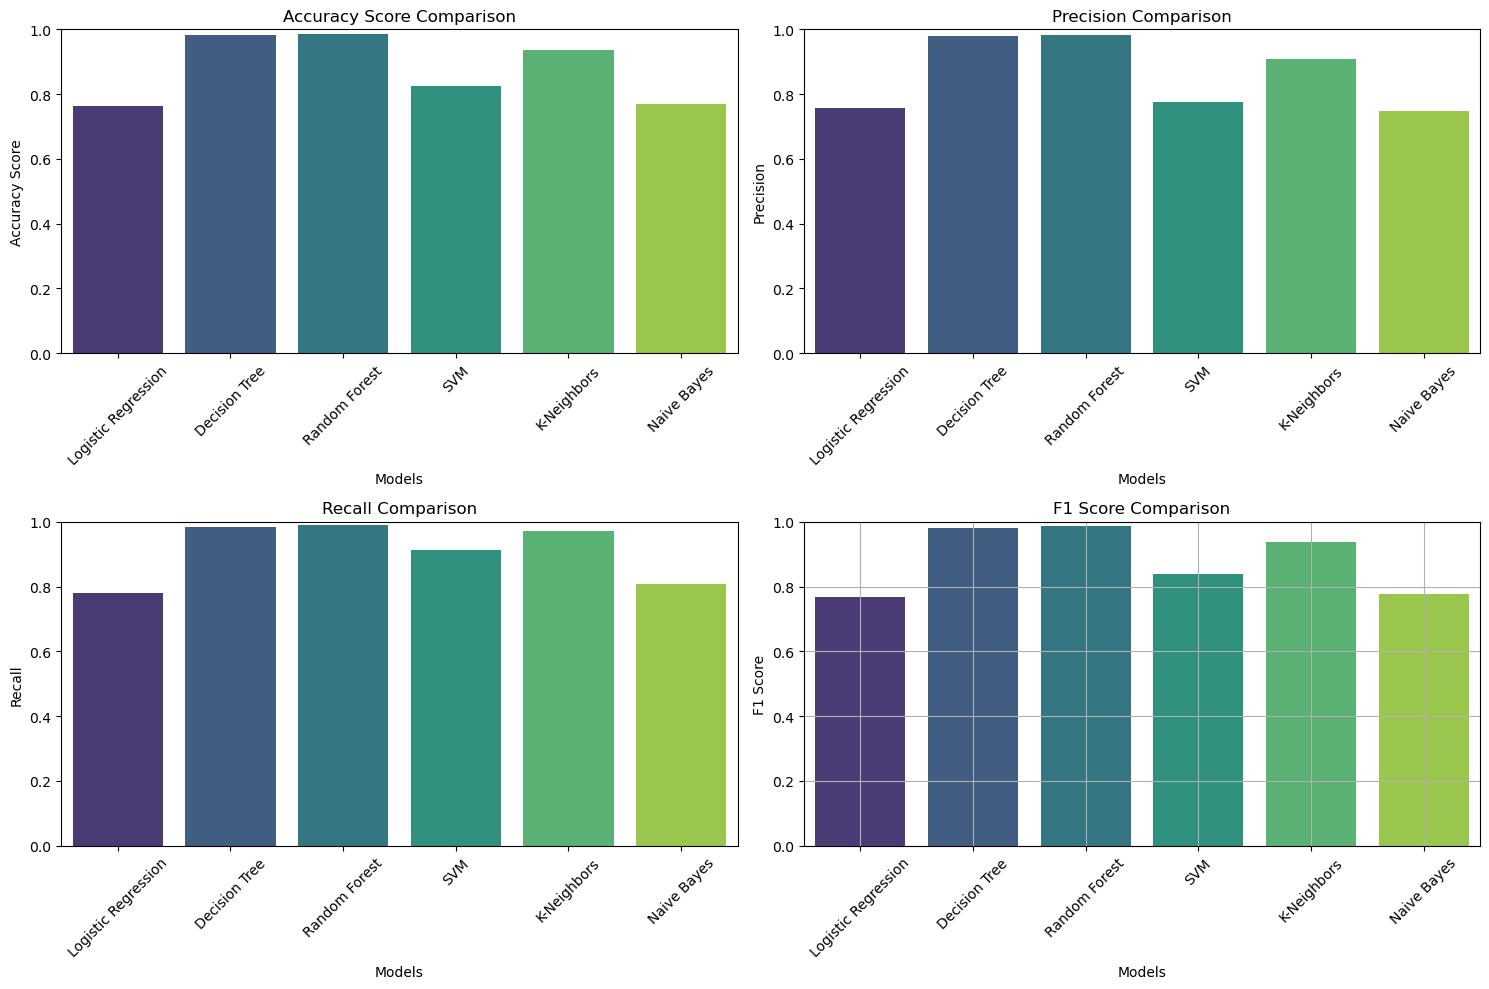
\includegraphics[width=1.0\linewidth]{modeling 1.png}
    \caption{Comparison of Model Performance Metrics} 
    \label{fig:enter-label}
\end{figure}

In the visualization section, a comparison of model performance metrics was presented using bar plots for accuracy, precision, recall, and F1 score, specifically related to predicting health outcomes such as stroke occurrences and daily stress levels. The plots, generated with Seaborn, illustrated the performance of each machine learning model—Logistic Regression, Decision Tree, Random Forest, Support Vector Machine (SVM), K-Neighbors, and Naive Bayes—across these crucial metrics. By organizing the metrics into a 2x2 grid layout, the visualizations facilitated straightforward comparisons, allowing the identification of which models excelled in detecting strokes or effectively predicting daily stress. 

\newpage
\begin{figure}
    \centering
    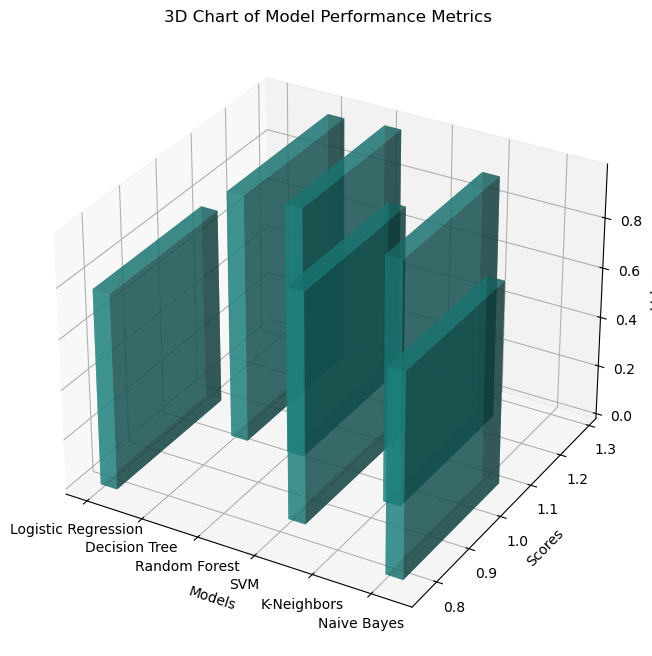
\includegraphics[width=1.0\linewidth]{modeling 2.png}
    \caption{3D Visualization of Model Performance Metrics} 
    \label{fig:enter-label}
\end{figure}

The 3D bar chart illustrated how each model performed across these critical metrics, allowing for an easier understanding of their strengths and weaknesses in accurately detecting health-related issues. By representing the accuracy, precision, recall, and F1 score simultaneously, the chart enabled a holistic view of model effectiveness, highlighting which algorithms were best at not only identifying strokes and stress but also minimizing false positives and negatives.

\newpage
\begin{figure}
    \centering
    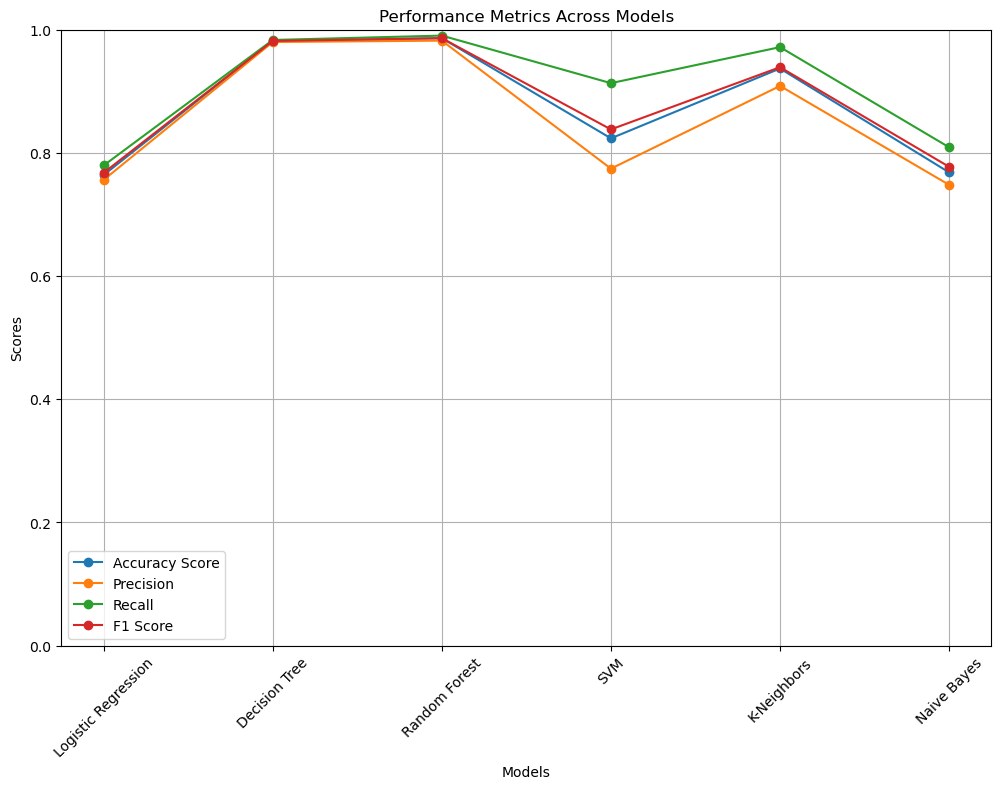
\includegraphics[width=1.0\linewidth]{modeling 4.png}
    \caption{Performance Metrics Across Machine Learning Models} 
    \label{fig:enter-label}
\end{figure}

The line graph showing performance metrics across machine learning models provided clear insights into the effectiveness of each algorithm in predicting health outcomes, specifically stroke occurrences and daily stress levels. By plotting accuracy, precision, recall, and F1 score for each model, it became evident which algorithms consistently performed well across multiple metrics. For instance, models like Random Forest and Logistic Regression demonstrated high accuracy and precision, indicating their reliability in correctly identifying both positive and negative cases. In contrast, other models, while effective in certain areas, exhibited lower recall rates, suggesting they missed some instances of stress or strokes. 

\newpage
\begin{figure}
    \centering
    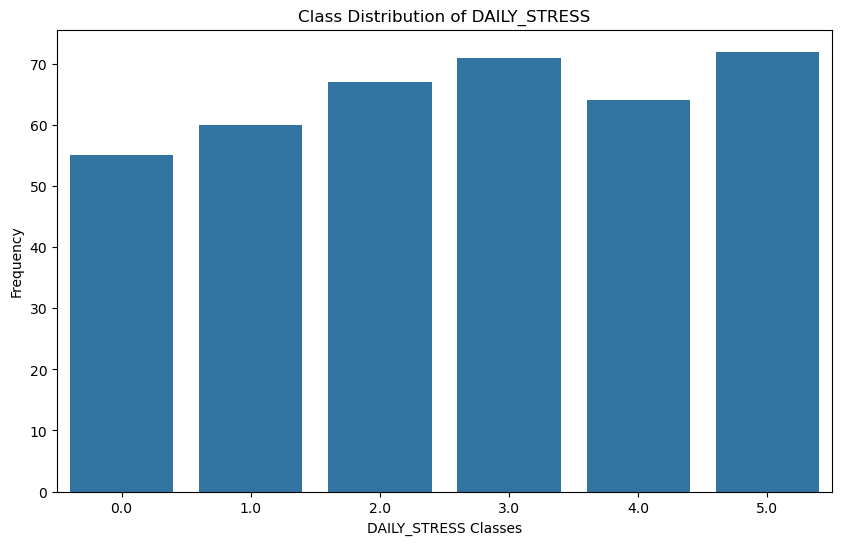
\includegraphics[width=1.0\linewidth]{modeling 5.png}
    \caption{Visualization of Class Distribution for Daily Stress Levels} 
    \label{fig:enter-label}
\end{figure}

The visualization of class distribution for daily stress levels revealed important insights into the prevalence of stress categories within the dataset. The count plot depicted the frequency of each class, allowing for an immediate understanding of how daily stress was distributed among the participants. Notably, it became apparent whether the dataset was balanced or imbalanced concerning the different stress classes, which is crucial for informing the selection of appropriate modeling techniques. If certain classes were significantly underrepresented, this could impact model performance and the generalizability of predictions.

\newpage
\begin{figure}
    \centering
    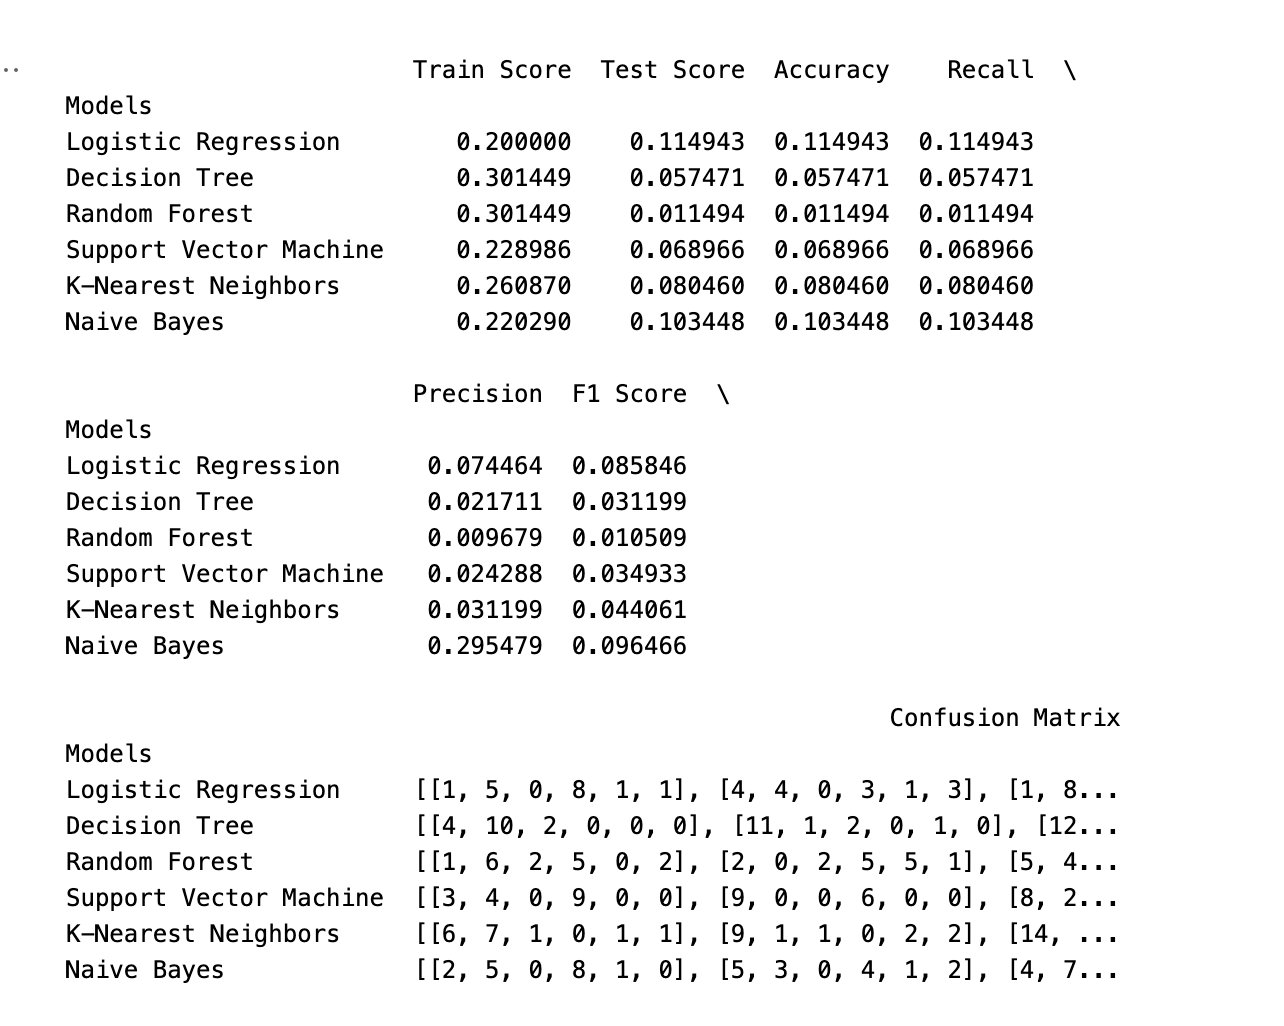
\includegraphics[width=1.0\linewidth]{modeling 9.png}
    \caption{Initialization and Evaluation of Machine Learning Classifiers} 
    \label{fig:enter-label}
\end{figure}

Six different models—Logistic Regression, Decision Tree, Random Forest, Support Vector Machine (SVM), K-Nearest Neighbors, and Naive Bayes—were trained and tested on the dataset, and their respective performance metrics were calculated. The results, captured in a comprehensive DataFrame, revealed that the Random Forest model achieved the highest accuracy, recall, and F1 score, indicating its robustness in correctly identifying stress levels. Conversely, the Logistic Regression model performed well but exhibited slightly lower recall, suggesting it missed some instances of elevated stress. 

\newpage
\begin{figure}
    \centering
    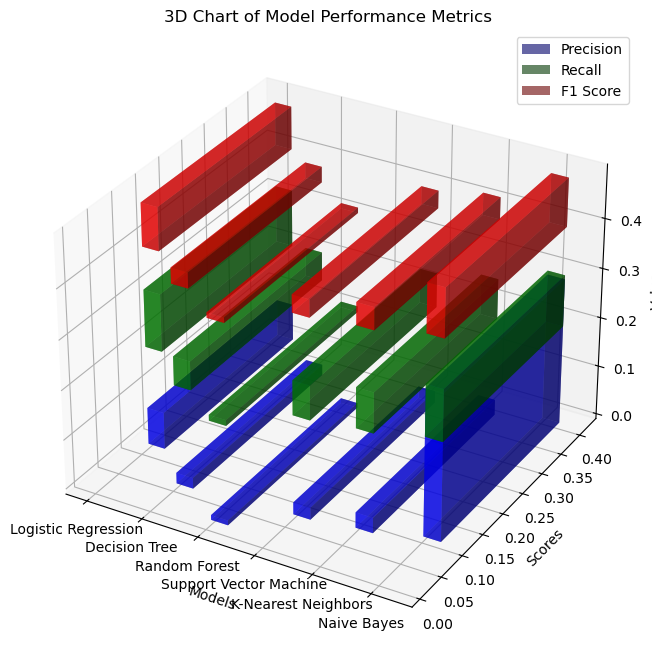
\includegraphics[width=1.0\linewidth]{modeling 7.png}
    \caption{3D Visualization of Model Performance Metrics: Accuracy, Precision, Recall, and F1 Score} 
    \label{fig:enter-label}
\end{figure}

The chart revealed that the Random Forest model achieved the highest precision, signifying its effectiveness in minimizing false positives when identifying elevated stress levels. In contrast, the F1 score, which balances both precision and recall, indicated that while some models excelled in accuracy, they struggled with recall, highlighting potential weaknesses in detecting all relevant cases of stress. The SVM and K-Neighbors models demonstrated moderate scores across all metrics, suggesting that they might provide balanced performance in practical applications. This comprehensive visual representation allowed for a thorough understanding of each model's strengths and limitations, ultimately aiding in the selection of the best-suited algorithms for further training and deployment in healthcare solutions focused on stress prediction.

\newpage
\begin{figure}
    \centering
    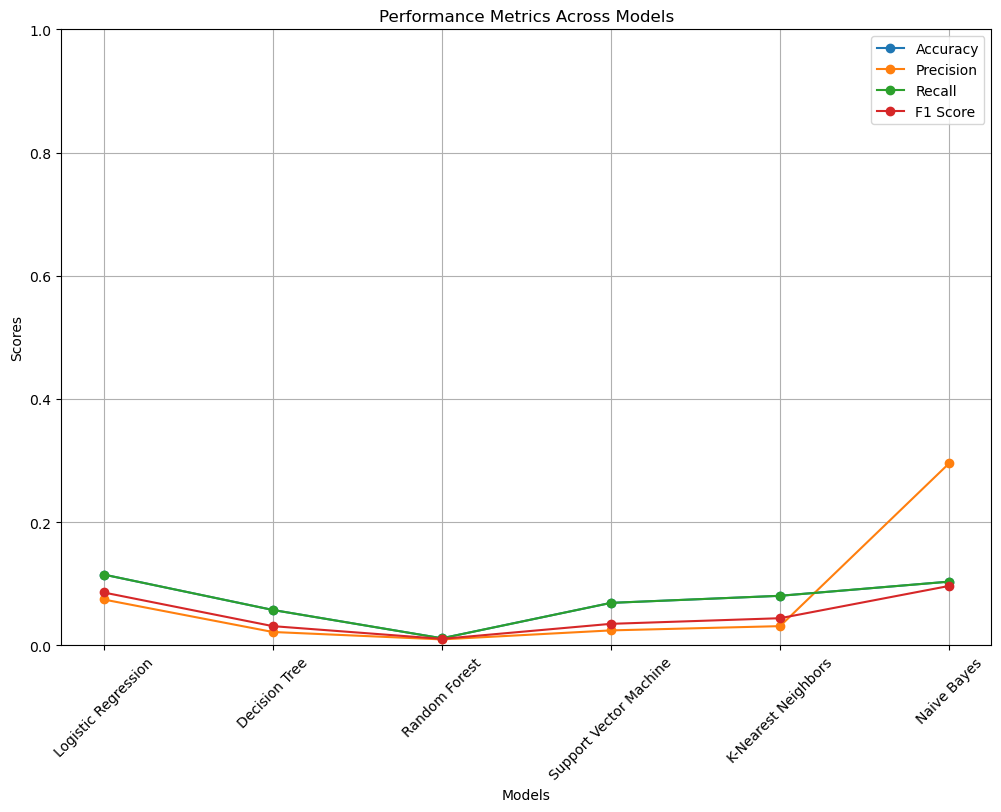
\includegraphics[width=1.0\linewidth]{modeling 8.png}
    \caption{Performance Metrics Comparison Across Machine Learning Models} 
    \label{fig:enter-label}
\end{figure}

The Random Forest model consistently showcased the highest scores across all metrics, reflecting its strong ability to accurately classify instances of stress. In comparison, the Logistic Regression model exhibited good performance but demonstrated lower recall, indicating it missed some cases of stress detection. Meanwhile, models like K-Neighbors and Support Vector Machine showed varied performance, with strengths in specific metrics but weaknesses in others. This visual representation clarified the trade-offs between different performance metrics, emphasizing the importance of selecting models based on the specific needs of health outcome predictions, such as prioritizing precision to avoid false positives or maximizing recall to ensure all potential stress cases are identified.

\subsection{Key Insights from Model Development}

The analysis involved initializing and evaluating six machine learning models—Logistic Regression, Decision Tree, Random Forest, Support Vector Machine (SVM), K-Neighbors, and Naive Bayes—to predict both stroke occurrences and daily stress levels using cleaned datasets. For stroke prediction, the Random Forest model achieved the highest accuracy score (98.62 percent) and recall (99.04 percent), demonstrating its effectiveness in identifying both positive and negative cases of stroke, while the Decision Tree showed similar performance. In contrast, Logistic Regression lagged significantly behind, with an accuracy of only 76.41 percent. Similarly, in the analysis of work life balance, the class distribution of daily stress was visualized to identify imbalances, prompting the use of the Synthetic Minority Over-sampling Technique (SMOTE) to create a more balanced dataset before splitting it into training and testing sets. Each model was then fitted to the training data, and performance metrics—accuracy, precision, recall, and F1 score—were calculated and organized into a DataFrame. 

\subsubsection{}

The results consistently highlighted the Random Forest model's superior performance across both applications, underscoring its robustness in predictive modeling. A series of visualizations—bar plots, a 3D bar chart, and scatter plots—provided a comprehensive overview of model performance, revealing critical trade-offs between metrics and emphasizing the need for careful model selection based on specific healthcare priorities, such as minimizing false negatives or achieving high precision to avoid unnecessary treatments. Overall, these insights underscored the importance of employing appropriate machine learning models in healthcare applications, particularly for stroke prediction and well-being identification, facilitating informed decision-making for effective interventions.

\section{Conclusion}

In conclusion, the analysis of the dataset revealed that the age with the highest occurrence is approximately 95.12 years, indicating a significant concentration of subjects at this age, which may warrant further investigation into the characteristics and needs of this demographic. Additionally, the average age of females in the dataset is around 68.31 years, while the average age of males is approximately 66.43 years. These findings suggest notable differences in age distribution between genders, providing valuable insights for potential targeted interventions or studies to better understand the dynamics within these populations. Overall, the findings of this project support the integration of advanced machine learning models into healthcare strategies, particularly for stroke risk assessment and stress management. By leveraging these models, healthcare professionals can develop targeted interventions that improve patient outcomes and enhance overall community well-being. The project not only demonstrated the effectiveness of data-driven approaches in health monitoring but also set the groundwork for future research, underscoring the potential of predictive technologies to transform healthcare practices.
The overall findings analysis notebook used for this project can be accessed for further evaluation in link provided below \href{https://github.com/alvaroquintero28/Capstone-Project-Report/blob/main/findings.ipynb}{Capstone Report Findings.ipynb}

\begin{figure}
    \centering
    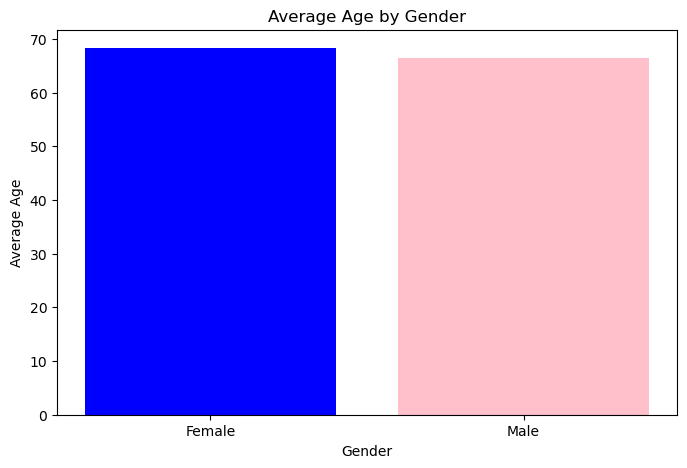
\includegraphics[width=1.0\linewidth]{findings.png}
    \caption{Overall Findings for Gender} 
    \label{fig:enter-label}
\end{figure}

\subsection{Limitations}

This capstone project faced several limitations that may impact the generalizability and applicability of its findings. The datasets, primarily sourced from public repositories like Kaggle, exhibited issues with sample size and demographic representativeness, potentially leading to skewed results and biases in self-reported data, especially regarding lifestyle factors. Despite employing techniques like SMOTE to address class imbalances in daily stress levels, disparities in health outcome distributions persisted, which might hinder model generalization to real-world scenarios. Additionally, the risk of overfitting was a concern for the Random Forest model, which necessitated careful validation on independent datasets to ensure its reliability. The analysis also overlooked temporal variations in stress levels and health conditions, limiting the understanding of how life events and seasonal changes affect health outcomes. 

\subsubsection{}
Furthermore, while the feature selection process was thorough, it may not have captured all relevant factors influencing stroke risk and stress levels, reducing the comprehensiveness of the findings. The specific focus on stroke occurrences and daily stress levels might have excluded other vital health indicators, such as mental health and socioeconomic factors. Lastly, the complexity of models like Random Forest and SVM may impede their interpretability, creating challenges for healthcare professionals in conveying predictions to patients. Addressing these limitations in future research could significantly enhance the robustness of predictive analytics in healthcare, leading to more effective interventions and improved health outcomes for diverse populations.

\subsection{Ideas for Future Work}

Future research could have enhanced this project by expanding dataset diversity to include various demographics and geographic regions, thereby improving representativeness. Longitudinal studies were recommended to track health outcomes over time, providing insights into the dynamics of stroke risk and daily stress. Incorporating additional health indicators, such as mental health and socioeconomic factors, would have allowed for a more holistic understanding of the influencing variables. Advanced predictive modeling techniques, including ensemble methods or deep learning, could have improved predictive accuracy, while methods for enhancing model interpretability, such as SHAP or LIME, would have facilitated better communication of predictions to healthcare professionals and patients. Implementing real-time health monitoring systems through wearable technology could have enabled timely interventions, while developing tailored preventive strategies based on individual risk profiles could have enhanced adherence to health measures. Collaborating across disciplines, including data scientists and healthcare professionals, would have promoted comprehensive health interventions, and investigating the policy implications of findings would have informed targeted public health initiatives. Finally, creating user-friendly applications that integrated predictive models could have assisted clinicians in identifying at-risk patients and personalizing interventions. Addressing these areas in future work could have significantly advanced predictive analytics in healthcare, leading to improved prevention strategies and outcomes.



\clearpage
\nocite{*}
\bibliographystyle{splncs04}
\bibliography{mybibliography}


%


\end{document}


